\chapter{ハドロンのレッジェ軌道から光円錐弦へ}

\lectureoverview{弦理論は量子重力の理論として始まったのではない。
それはハドロンのスペクトルと散乱を理解しようとする試みとして始まった。
まっすぐなレッジェ軌道は拡がった対象を示唆し、パイオン--パイオン散乱における双対性は、一見異なる二つの過程が一つの曲面の二つの切り方であることを示唆した。われわれはそれらの手がかりを追って世界面の描像へ進み、ハドロン弦をQCDのフラックスチューブとして再解釈し、次に無限運動量枠を用いて開弦の横方向の力学を導く。中心的な結果は、その有効内部ハミルトニアンが質量の二乗を測るということである。したがって、その記述において\(L^2\)に比例するフックの法則のエネルギーは、\(L\)に比例する静止エネルギーとなり、これは一定の張力をもつ弦の定義的な振る舞いである。}

\section{弦理論のハドロン的起源}

1968年--1970年ごろ、弦理論へと導いた問題は陽子、中性子、とりわけ中間子に関するものであった。クォーク模型はすでに真剣な考え方であったが、ハドロンのクォーク内容は現代的な意味でまだ実験的に確立されていなかった。グルーオンは通常の議論ではさらに目立たなかった。南部は関連するゲージ場の考えを提案していたが、量子色力学の定まった言葉はまだ存在しなかった。代わりに素材となったのは、予想外に豊かな強く相互作用する粒子のスペクトルであった。

陽子--中性子の区別を一時的に無視し、両方の状態を核子と呼ぶと便利である。核子の先にはより大きなスピンをもつより重い状態があり、さらにその先にはさらに大きなスピンをもつさらに重い状態が続いた。ChewとFrautschiはそのような家族を、縦軸に角運動量、横軸に質量の二乗をとった図の上に整理した。当時の歴史的な単位では陽子の質量は約1 BeVであり、同じ単位は現在GeVと呼ばれている。

角運動量を\(\hbar\)の単位で測る。バリオンの家族では、無次元のスピンの値は半整数であり、

\begin{equation}
  J=\frac12,\frac32,\frac52,\ldots,
\end{equation}

一方、中間子の家族は整数スピンをもつ。驚くべき経験的事実は、どちらの家族も\(M^2\)に対してプロットするとほぼ直線上に並ぶということであった。現代的な記法では次のように書く。

\begin{equation}
  J\simeq \alpha_0+\alpha' M^2,
  \label{eq:l01-regge-trajectory}
\end{equation}

ここで\(\alpha_0\)は切片であり、\(\alpha'\)はレッジェ傾斜である。
\editorialnote{この講義は観測された線形関係とそのほぼ普遍的な傾斜を強調している。切片の記法はその関係を簡潔に述べるためにのみ与えられており、軌道は経験的かつ近似的なものである。}

最初の直線は、既知の二点しか通っていなかったため説得力がなかった。任意の二点は一つの直線を定める。驚きは後に訪れた。新たに発見された状態が同じ直線の近くに次々と並んだのである。中間子の軌道も同じ整理を示した。パイオンは\(J=0\)の近くでGeVスケールの小さな質量をもって始まり、ローは\(J=1\)で始まり、さらなる励起状態が上へと続く。一つの家族に五つ、六つ、あるいは七つの状態が現れることもあった。さらに驚くべきことに、異なるバリオンと中間子の軌道はほぼ平行であった。したがって、角運動量が一量子分増えることは、質量の二乗がほぼ同じ分だけ増えることに対応した。

\begin{equation}
  \Delta J=1
  \quad\Longrightarrow\quad
  \Delta M^2\simeq \frac{1}{\alpha'}.
  \label{eq:l01-regge-spacing}
\end{equation}

\begin{classroomqa}
\audiencequestion{異なるレッジェ軌道が平行であるとはどういう意味か。\lecturetimestamp{00:09:32}}
\lecturerresponse{一つの粒子の家族を選び、その励起状態をすべてプロットすると、それらは一つの直線上に並ぶ。これを別の中間子やバリオンの家族について繰り返す。切片は異なるにもかかわらず、直線はほぼ同じ傾斜をもつ。したがって、角運動量の同じ増分は、ほぼ同じ\(M^2\)の増分を要する。この共通の傾斜は普遍的なレッジェ傾斜と呼ばれた。}
\end{classroomqa}

普通の拡がった対象との比較は、なぜこのパターンが重要であったかを示す。バスケットボールは回転させられると回転エネルギーを得るが、その軌道は直線ではなく曲がっており、十分に高い角速度ではボールは引き裂かれる。原子も回転励起をもつが、やがてイオン化し、その軌道は終わる。ハドロンははるかに単純な系列を示し、利用可能なデータの範囲内では、その系列が尽きる兆しはなかった。

このスペクトルは、ハドロンが点のように振る舞っていないことを示していた。点には回転したり変形したりする空間的構造がない。電子には観測された高スピン内部状態の塔がなく、それに対応して現在の実験的限界の範囲内では点的である。対照的に、ハドロンは回転させることができる。そのスペクトルは複合性を示唆し、スピンと質量の関係は、角運動量が増えるにつれて対象が変形することを示唆する。

\section{パイオン--パイオン散乱における双対性}

分光は一つの手がかりを与えた。パイオン--パイオン散乱はもう一つの手がかりを与えた。二つのパイオンはロー的な共鳴状態に結合し、後に再び二つのパイオンとして現れることができる。従来のファインマン図では、これは消滅と再生成の過程であり、慣例的に\(s\)チャネル過程と呼ばれる。同じ基本図を横向きにすると、交差した、すなわち\(t\)チャネル過程が得られ、そこではロー的な粒子がパイオン間で交換される。

ローは単独ではない。それはレッジェ族に属するので、整合性のためにはどちらのチャネルにおいてもローとそのすべての励起パートナーが必要であるように思われる。概略的には、

\begin{equation}
  \mathcal A(s,t)\simeq
  \sum_n \mathcal A^{(s)}_{\rho_n}(s,t),
  \qquad
  \mathcal A(s,t)\simeq
  \sum_n \mathcal A^{(t)}_{\rho_n}(s,t).
  \label{eq:l01-channel-sums}
\end{equation}

これらの表式は単に足し合わせるべき二つの近似ではない。数値的研究により、消滅チャネルにおける共鳴の塔を足し合わせるだけで、交換チャネルから期待される寄与とほぼ同じものが得られることが分かった。逆に、交換される塔は共鳴の記述を再現することができた。したがって、両方の完全な塔を加えることは同じ物理を二重に数えているように思われた。通常の摂動的な帳簿付けでは、二つの図が存在するなら両方を含めなければならない。しかしハドロン振幅は、二つのチャネルの記述が双対であることを示唆していた。

\begin{figure}[H]
  \centering
  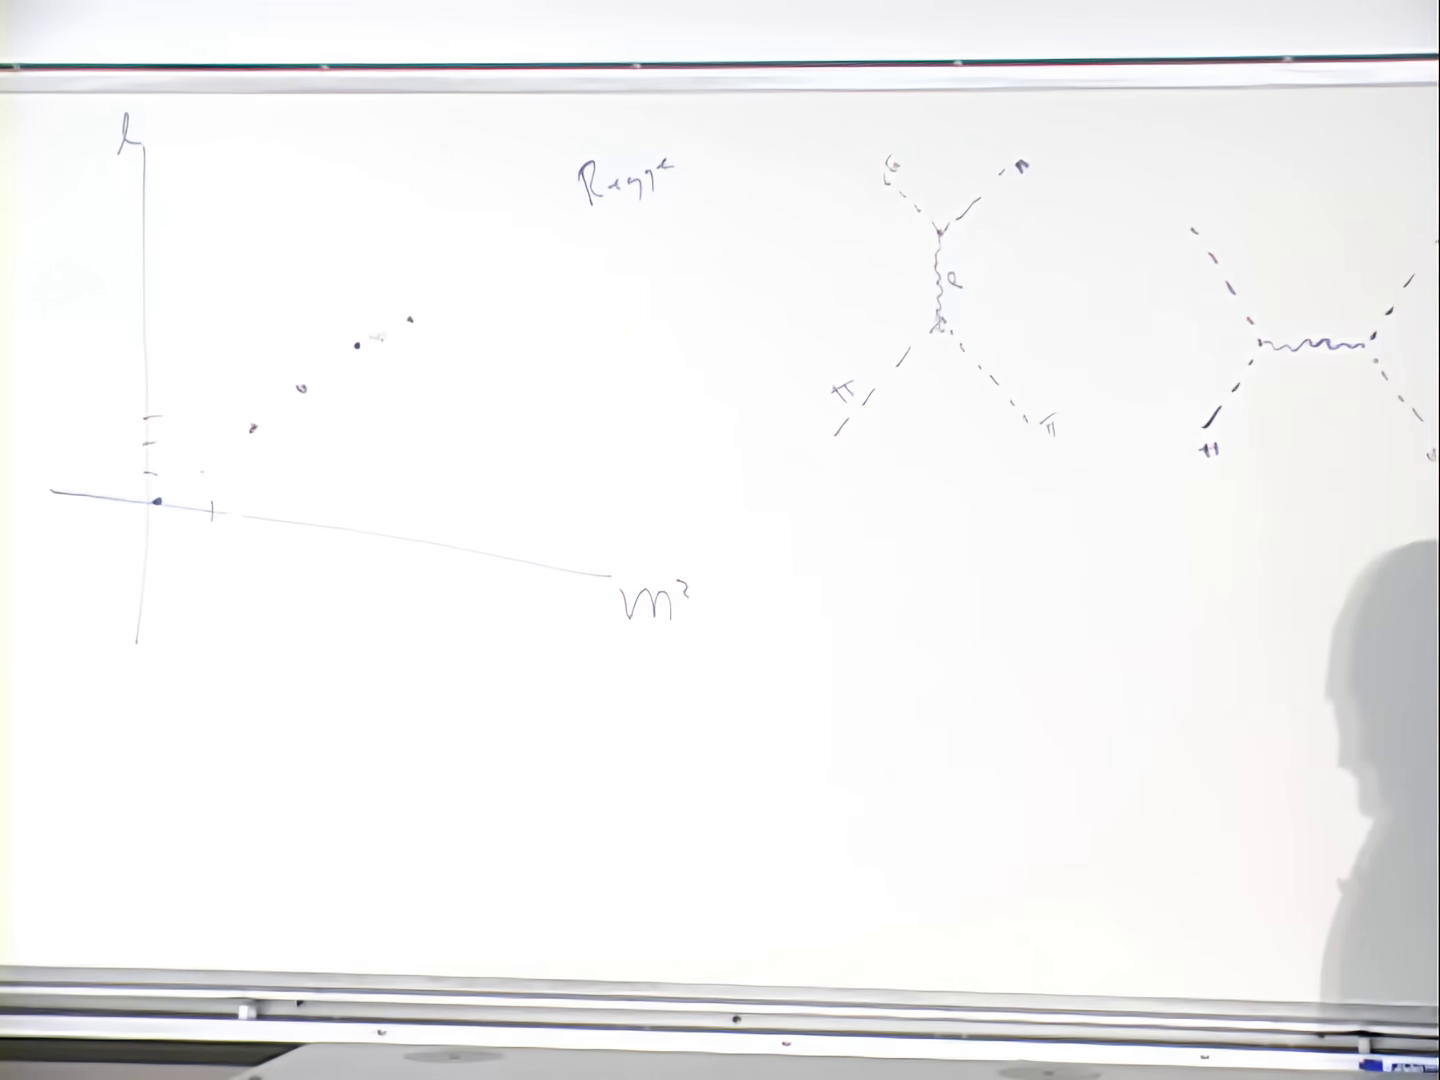
\includegraphics[width=0.82\textwidth]{lecture_01_figure_01.png}
  \caption{この板書はChew--Frautschiプロットを消滅チャネルと交差チャネルの図に結びつけ、スペクトルと散乱の手がかりを一つの問題の一部としている。}
  \lectureframe{00:14:20}
  \label{fig:l01-regge-duality-board}
\end{figure}

同じ関係は、明快な概略図に分けることができる。最初のパネルは線形スペクトルを記録し、他の二つは同じ振幅の代替チャネル展開を表している。

\begin{figure}[H]
  \centering
  \resizebox{\textwidth}{!}{%
  \begin{tikzpicture}[>=Latex,thick]
    \begin{scope}
      \draw[->] (0,0) -- (4.2,0) node[right] {$M^2$};
      \draw[->] (0,0) -- (0,3.4) node[above] {$J$};
      \draw[blue!65!black] (0.45,0.35) -- (3.55,2.95);
      \draw[orange!80!black] (0.75,0.20) -- (3.85,2.80);
      \foreach \x/\y in {0.65/0.52,1.35/1.10,2.05/1.69,2.75/2.27,3.45/2.86}
        \fill[blue!65!black] (\x,\y) circle (0.07);
      \foreach \x/\y in {0.95/0.37,1.65/0.95,2.35/1.54,3.05/2.12,3.75/2.71}
        \fill[orange!80!black] (\x,\y) circle (0.07);
      \node at (2.1,-0.55) {parallel Regge families};
    \end{scope}
    \begin{scope}[xshift=5.7cm]
      \draw[->] (-1.5,1.2) -- (-0.3,0.25);
      \draw[->] (-1.5,-1.2) -- (-0.3,-0.25);
      \draw[decorate,decoration={snake,amplitude=1.5pt,segment length=7pt}]
        (0,0.25) -- (0,-0.25);
      \draw[->] (0.3,0.25) -- (1.5,1.2);
      \draw[->] (0.3,-0.25) -- (1.5,-1.2);
      \node at (0,-1.75) {$s$-channel tower};
    \end{scope}
    \begin{scope}[xshift=10.5cm]
      \draw[->] (-1.5,1.2) -- (1.5,1.2);
      \draw[->] (-1.5,-1.2) -- (1.5,-1.2);
      \draw[decorate,decoration={snake,amplitude=1.5pt,segment length=7pt}]
        (0,0.95) -- (0,-0.95);
      \node at (0,-1.75) {$t$-channel tower};
    \end{scope}
  \end{tikzpicture}}
  \caption{平行なレッジェ族と、ハドロン双対性に関与する二つのチャネル展開。}
  \label{fig:l01-regge-duality-redraw}
\end{figure}

\section{一つの世界面、二つの切断}

自然な応答は、どちらのようにも読める一つの幾何学的歴史を探すことであった。パイオンをクォーク--反クォーク対で表し、時間を上向きに走らせる。一次元の粒子線だけを描く代わりに、クォークの軌跡で囲まれた領域を埋める。この二次元の歴史を横に切った断面は、二つの入射弦が結合し、後に分離することを示すかもしれない。別の切断は、一方の側から他方の側へ交換される弦を表示する。二つのファインマンチャネルの絵はもはや独立した機構ではなく、一つの面の異なる分解である。

\begin{figure}[H]
  \centering
  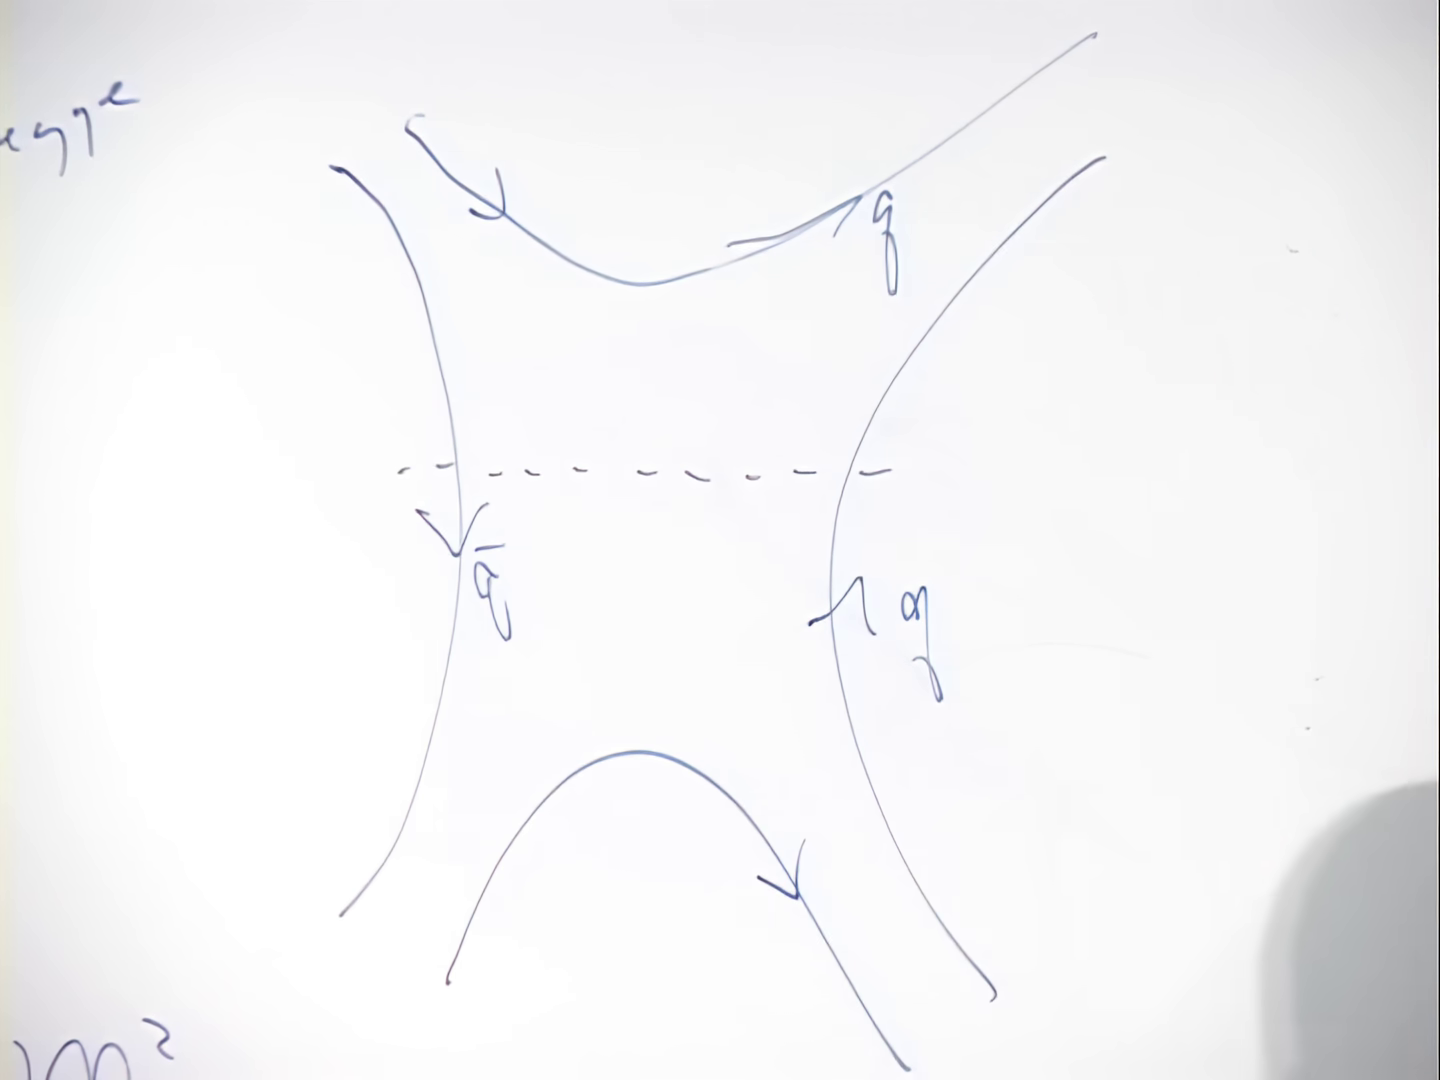
\includegraphics[width=0.78\textwidth]{lecture_01_figure_02.png}
  \caption{板書上のクォーク線のトポロジー。同じ二次元の歴史を通る異なる切断が、共鳴と交換の読みを与える。}
  \lectureframe{00:17:50}
  \label{fig:l01-worldsheet-topology-board}
\end{figure}

クォークと反クォークの間の領域は、さらにもう一つの考えを与える。固定された時刻において、断面は二つの端点と、それらの間の全区間を埋める何かを含む。その対象は一次元である。すなわち弦である。相互作用の間、弦は二次元の面を掃き出す。

\begin{definition}
点粒子の時空の歴史は\emph{世界線}である。弦の時空の歴史は\emph{世界面}である。ある瞬間の弦は、その世界面の空間的断面である。
\end{definition}

\begin{figure}[H]
  \centering
  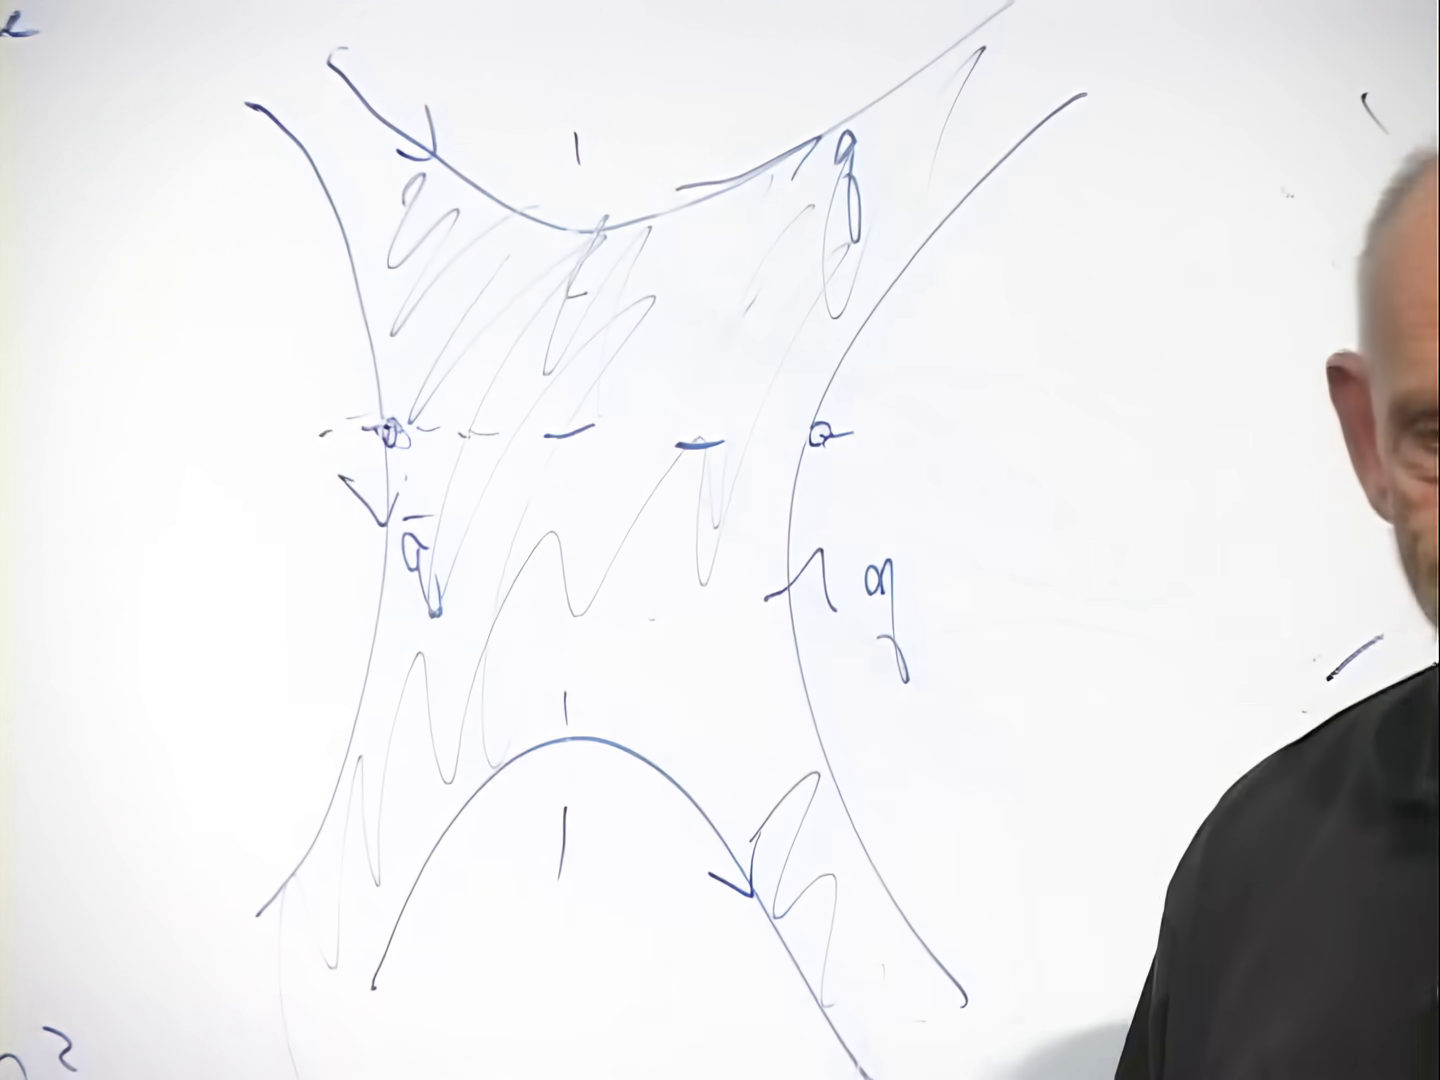
\includegraphics[width=0.78\textwidth]{lecture_01_figure_03.png}
  \caption{端点の軌跡の間に埋められた板書の面。時間断面はそれを一次元の弦で交差する。}
  \lectureframe{00:19:15}
  \label{fig:l01-worldsheet-filled-board}
\end{figure}

\begin{figure}[H]
  \centering
  \begin{tikzpicture}[>=Latex,scale=0.95]
    \fill[blue!10]
      (-2.6,-2.3) .. controls (-1.0,-1.0) and (-1.0,-0.4) .. (-0.2,0)
      .. controls (-1.0,0.5) and (-1.0,1.0) .. (-2.6,2.3)
      -- (2.6,2.3)
      .. controls (1.0,1.0) and (1.0,0.5) .. (0.2,0)
      .. controls (1.0,-0.4) and (1.0,-1.0) .. (2.6,-2.3) -- cycle;
    \draw[blue!65!black]
      (-2.6,-2.3) .. controls (-1.0,-1.0) and (-1.0,-0.4) .. (-0.2,0)
      .. controls (-1.0,0.5) and (-1.0,1.0) .. (-2.6,2.3);
    \draw[blue!65!black]
      (2.6,-2.3) .. controls (1.0,-1.0) and (1.0,-0.4) .. (0.2,0)
      .. controls (1.0,0.5) and (1.0,1.0) .. (2.6,2.3);
    \draw[red!75!black,dashed] (-2.9,-1.15) -- (2.9,-1.15)
      node[right] {time slice};
    \draw[orange!80!black,dashed] (-1.55,-2.5) -- (1.55,2.5)
      node[above] {crossed slicing};
    \draw[->] (3.45,-1.7) -- (3.45,1.8) node[above] {time};
    \node[blue!65!black] at (0,-2.7) {one world sheet};
  \end{tikzpicture}
  \caption{明快な世界面の概略図。異なる切断が同じ面を異なる中間チャネルの記述に組織する。}
  \label{fig:l01-worldsheet-redraw}
\end{figure}

この幾何学的再構成は探索的なものであり、完全な理論を第一原理から演繹したものではなかった。初期の弦の描像には人によって異なる道から到達した。その強みは、同じ拡がった対象が両方の観測に対処できることであった。弦は回転し変形することができ、その世界面は双対な散乱チャネルを符号化することができる。

\begin{classroomqa}
\audiencequestion{なぜクォーク間で交換される通常の粒子ではなく、弦のような橋を導入するのか。\lecturetimestamp{00:21:20}}
\lecturerresponse{ある瞬間には、局在した交換粒子が存在するだけではない。クォーク、反クォーク、そしてそれらの間のすべての点における構造が存在する。その構造は根本的に連続であるかもしれないし、連続体を近似する密な構成要素の集まりであるかもしれない。最初の描像はそれを決定しなかった。重要だったのは、区間全体が占められており、観測された軌跡が両端に重りを付けた通常の靴ひものように終止する傾向を示さなかったことである。}
\end{classroomqa}

\begin{classroomqa}
\audiencequestion{標準模型はパイオン散乱を記述できるか？
\lecturetimestamp{00:22:45}}
\lecturerresponse{はい、ただしその有用性はエネルギー領域に依存する。低エネルギーでは、標準模型はQCDとその低エネルギー記述を通じて、パイオン散乱の多くを説明する。より高いエネルギーでは、ハドロン交換の塔全体が重要になり、直接計算はより困難になり、弦的な組織化の方がより有用でありうる。}
\end{classroomqa}

\begin{classroomqa}
\audiencequestion{初期の実験は、レッジェ軌跡が決して終わらないことを確立したのか？\lecturetimestamp{00:23:37}}
\lecturerresponse{いいえ。それらが確立したのは、観測された系列がまだ終点を示していないということだけである。無限に伸び続けるという推論は示唆的な外挿であり、測定された無限大ではない。}
\end{classroomqa}

\section{フラックス管とスケールの変化}

現代のQCDは、この古い描像に場の理論的な解釈を与える。クォークと反クォークはグルーオン場の反対向きの源として振る舞う。通常の電気力学では、反対符号の電荷を引き離すと電気フラックスは横方向に広がる。場は距離とともに弱まるので、電荷間の領域は固定した横断面プロファイルを保たない。QCDは非線形である。そのダイナミクスは、関連するクロモ電場フラックスをクォークと反クォークを結ぶ細い管に閉じ込めることができる。

\begin{figure}[H]
  \centering
  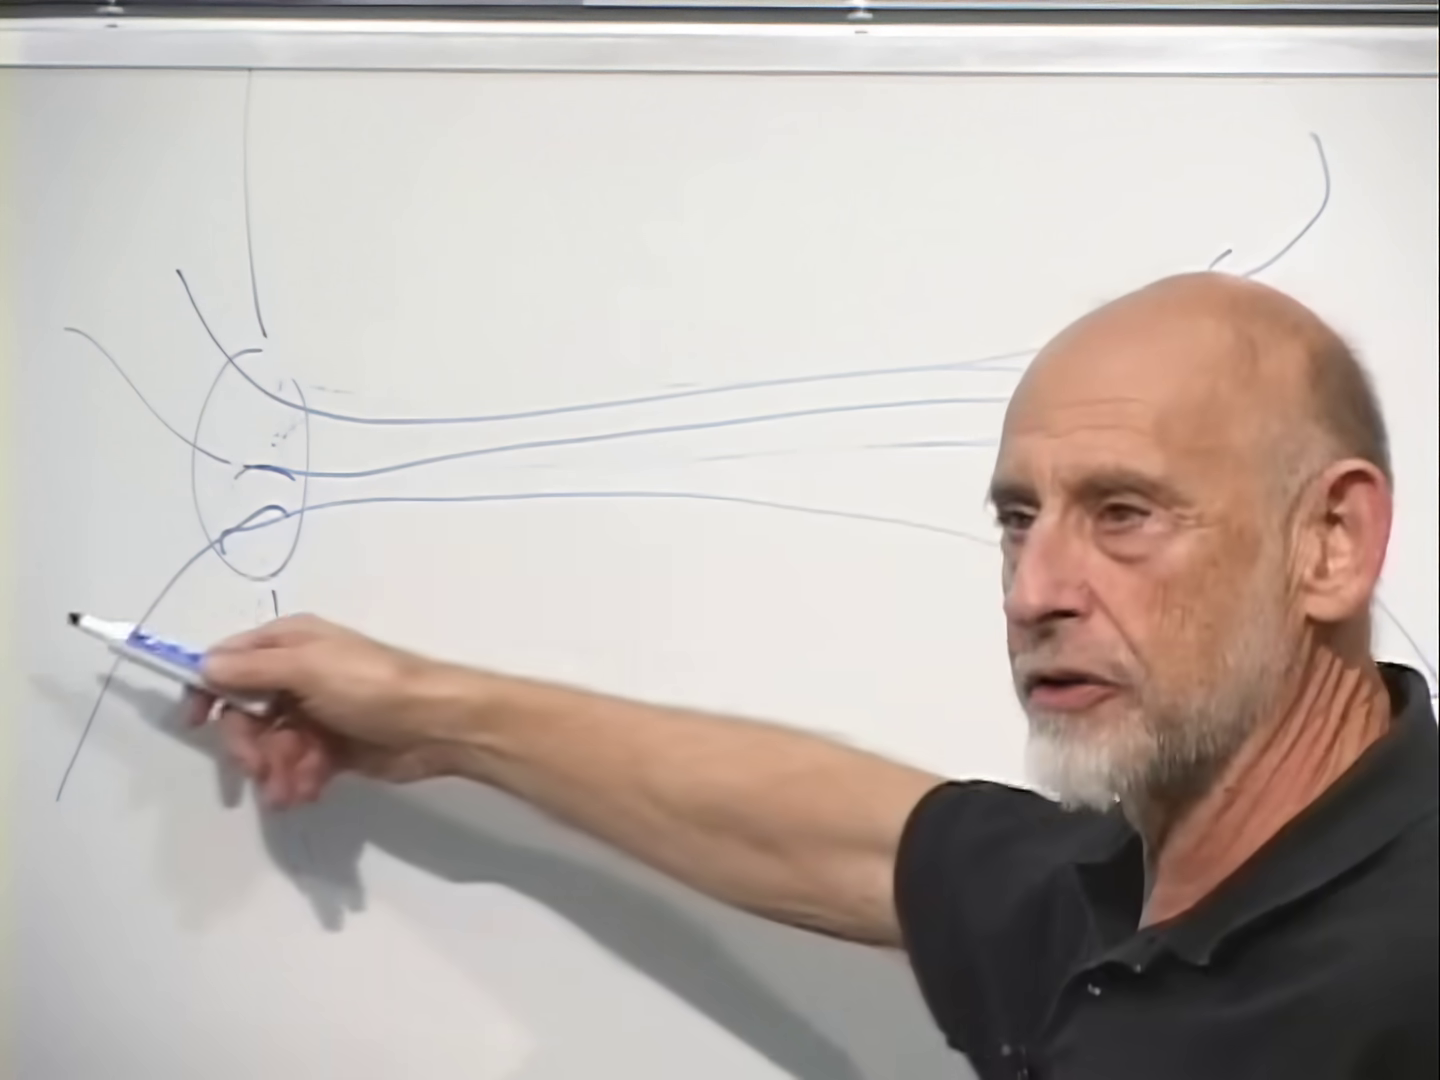
\includegraphics[width=0.78\textwidth]{lecture_01_figure_04.png}
  \caption{クォークと反クォークの場の線が、自由に広がるクーロン場ではなく、細いフラックス管として描かれている。}
  \lectureframe{00:25:15}
  \label{fig:l01-qcd-flux-board}
\end{figure}

\begin{figure}[H]
  \centering
  \begin{tikzpicture}[>=Latex]
    \fill[orange!14,rounded corners=8pt] (-3.0,-0.55) rectangle (3.0,0.55);
    \draw[orange!80!black,thick,rounded corners=8pt]
      (-3.0,-0.55) rectangle (3.0,0.55);
    \fill[blue!70!black] (-3.35,0) circle (0.17);
    \fill[red!75!black] (3.35,0) circle (0.17);
    \node[below] at (-3.35,-0.22) {$q$};
    \node[below] at (3.35,-0.22) {$\bar q$};
    \foreach \y in {-0.30,0,0.30}
      \draw[->,orange!85!black] (-3.05,\y) -- (3.05,\y);
    \draw[<->] (-2.9,-1.05) -- (2.9,-1.05) node[midway,below] {$L$};
    \node at (0,0.92) {approximately fixed transverse profile};
  \end{tikzpicture}
  \caption{閉じ込められたフラックス管は広がらずに長くなる。単位長さあたりのエネルギーが一定であることから\(E=TL\)が得られる。}
  \label{fig:l01-qcd-flux-redraw}
\end{figure}

粒子の言語と場の言語は、同じことを異なる仕方で述べている。場の記述では、管は端点が離れるにつれてほぼ同じ場の強さと断面積を保つ。構成要素の描像では、引き伸ばしのエネルギーが端点間にさらなるグルーオン構造を生み出す。通常のゴムバンドは分子の数が固定されているので、材料が破断するまで分子が離れていく。代わりに、隙間が開くたびに新しい分子が挿入されると想像してみよう。バンドに沿った密度は固定されたままで、バンドはより長くなりうる。これがグルーオン場に対する意図された類推である。管は破断に向かって細くなるのではなく、長さを増すのである。

\begin{classroomqa}
\audiencequestion{電子を構成する弦もグルーオンからできているのか？\lecturetimestamp{00:28:08}}
\lecturerresponse{そのような結論は導かれない。ハドロン弦は陽子のスケールにおけるQCDの対象である。量子重力に関係する仮想的な基本弦は、はるかに小さいプランクスケール付近に存在するであろうし、ここには電子がハドロンのグルーオン弦であるという証拠はない。注目すべき事実は、関連する数学が両方のスケールで現れたということであり、物理的対象が同一であるということではない。}
\end{classroomqa}

ハドロンの描像を完全な相互作用する弦理論に変えようとする試みは有望であったが、望ましいハドロン理論を完全に生み出すには至らなかった。その数学的模型には繰り返しスピン2の質量ゼロ粒子が含まれていた。ハドロン理論ではその状態は望ましくない予言のように見えたが、重力理論としてはまさにグラビトンの量子数を持っていた。Joel ScherkとJohn Schwarzは決定的な再解釈を行った。おそらくこの理論はハドロンではなく量子重力について語っているのだ、と。ハドロンへの応用と基本的な応用は物理的に異なるが、初期のハドロン問題が数学への道を与えたのである。

\begin{classroomqa}
\audiencequestion{フラックス線はどのように正の端点から負の端点へ向かうのか？\lecturetimestamp{00:31:46}}
\lecturerresponse{それらは一方の源を出て他方の源に入る。ちょうど磁力線が棒磁石のN極からS極へ向かうのと同じである。反対の端点のラベルはフラックスの向きを表しており、棒磁石も同様に二つのN極ではなく二つの反対の極を持つ。}
\end{classroomqa}

\begin{classroomqa}
\audiencequestion{弦は連続か離散か？
\lecturetimestamp{00:32:45}}
\lecturerresponse{量子論はその区別を微妙にする。電磁場は連続場として表され、同時に離散的な量子を持つ。同じように、弦は連続的に扱われながら、その励起は量子化されうる。問われている問題に応じて、両方の記述が有効でありうる。}
\end{classroomqa}

\begin{classroomqa}
\audiencequestion{世界面を切る時空のスライスの角度を変えた場合、その交わりは依然として弦なのか。\lecturetimestamp{00:34:20}}
\lecturerresponse{はい。同時性のスライスを変えることはローレンツ変換である。新しいスライスは、異なる運動状態にある弦としてその曲面と交わる。重心が静止している弦でさえ、内部的には静止していない。振動しうる。``静止''とは、その重心についてのみ言及している。}
\end{classroomqa}

\section{相対論的エネルギーの2つの展開}

広がりを持ち振動する物体を相対論的に直接記述するのは厄介である。有用な戦略は、その関連する運動が通常の非相対論的力学の形をとるような座標系を見つけることである。まず単一粒子から始める。非相対論的には次のように書く。

\begin{equation}
  E_{\mathrm{nr}}=\frac{\bm p^2}{2m}+B,
  \label{eq:l01-nonrel-energy}
\end{equation}

ここで\(B\)は全運動量に依存しない内部エネルギーまたは束縛エネルギーである。相互作用しない複数の粒子に対しては、運動項と内部定数の両方が加算される。運動を支配するのはエネルギー差のみであるから、状態に依存しない加法的定数はしばしば省略できる。

厳密な相対論的エネルギーは

\begin{equation}
  E=\sqrt{\bm p^2c^2+m^2c^4}.
  \label{eq:l01-rel-energy-c}
\end{equation}

\begin{figure}[H]
  \centering
  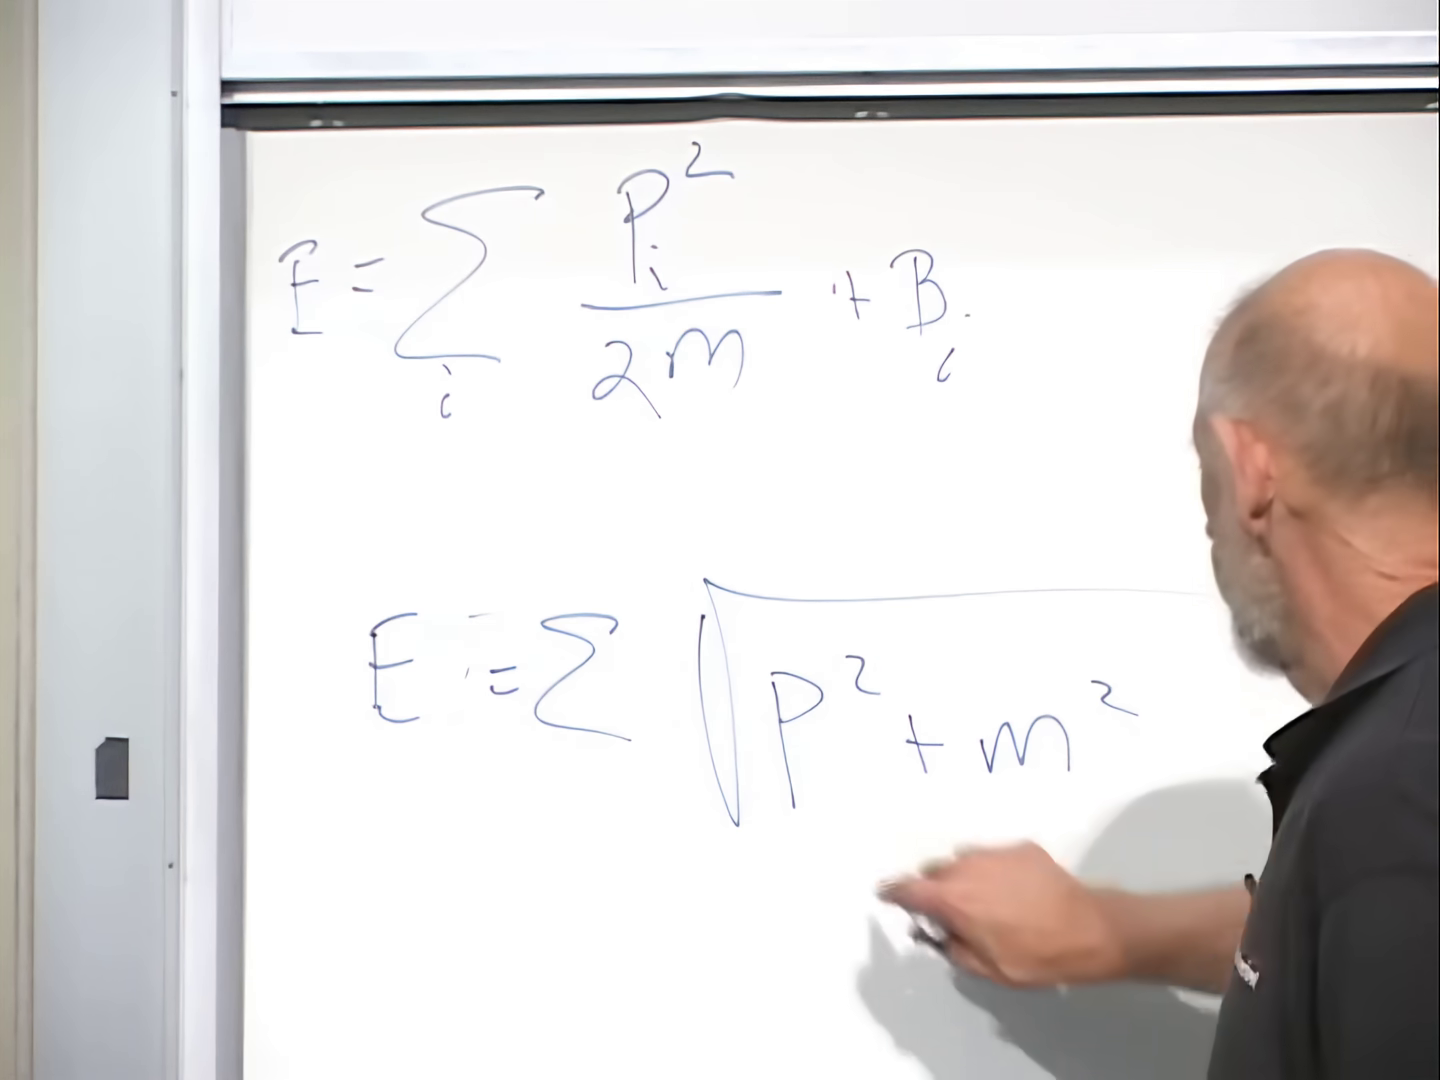
\includegraphics[width=0.76\textwidth]{lecture_01_figure_05.png}
  \caption{非相対論的運動エネルギーと厳密な相対論的平方根。議論の中で\(c\)の冪は修正される。}
  \lectureframe{00:38:45}
  \label{fig:l01-relativistic-energy-board}
\end{figure}

\begin{classroomqa}
\audiencequestion{相対論的公式は、最初に黒板に書かれた冪ではなく、\(p^2c^2\)と\(m^2c^4\)を含むべきではないか。\lecturetimestamp{00:39:12}}
\lecturerresponse{はい。次元の整合性により、式は\(E^2=p^2c^2+m^2c^4\)に固定される。非相対論的極限を回復した後で\(c=1\)と置くが、ここで冪を保っておくことで展開が透明になる。}
\end{classroomqa}

\(p^2c^2\ll m^2c^4\)のとき、\(m^2c^4\)をくくり出し、\(\sqrt{1+\epsilon}\simeq1+\epsilon/2\)を用いる。

\begin{align}
  E
  &=mc^2\sqrt{1+\frac{p^2}{m^2c^2}}
  \notag\\
  &\simeq mc^2+\frac{p^2}{2m}.
  \label{eq:l01-low-momentum-expansion}
\end{align}

\begin{figure}[H]
  \centering
  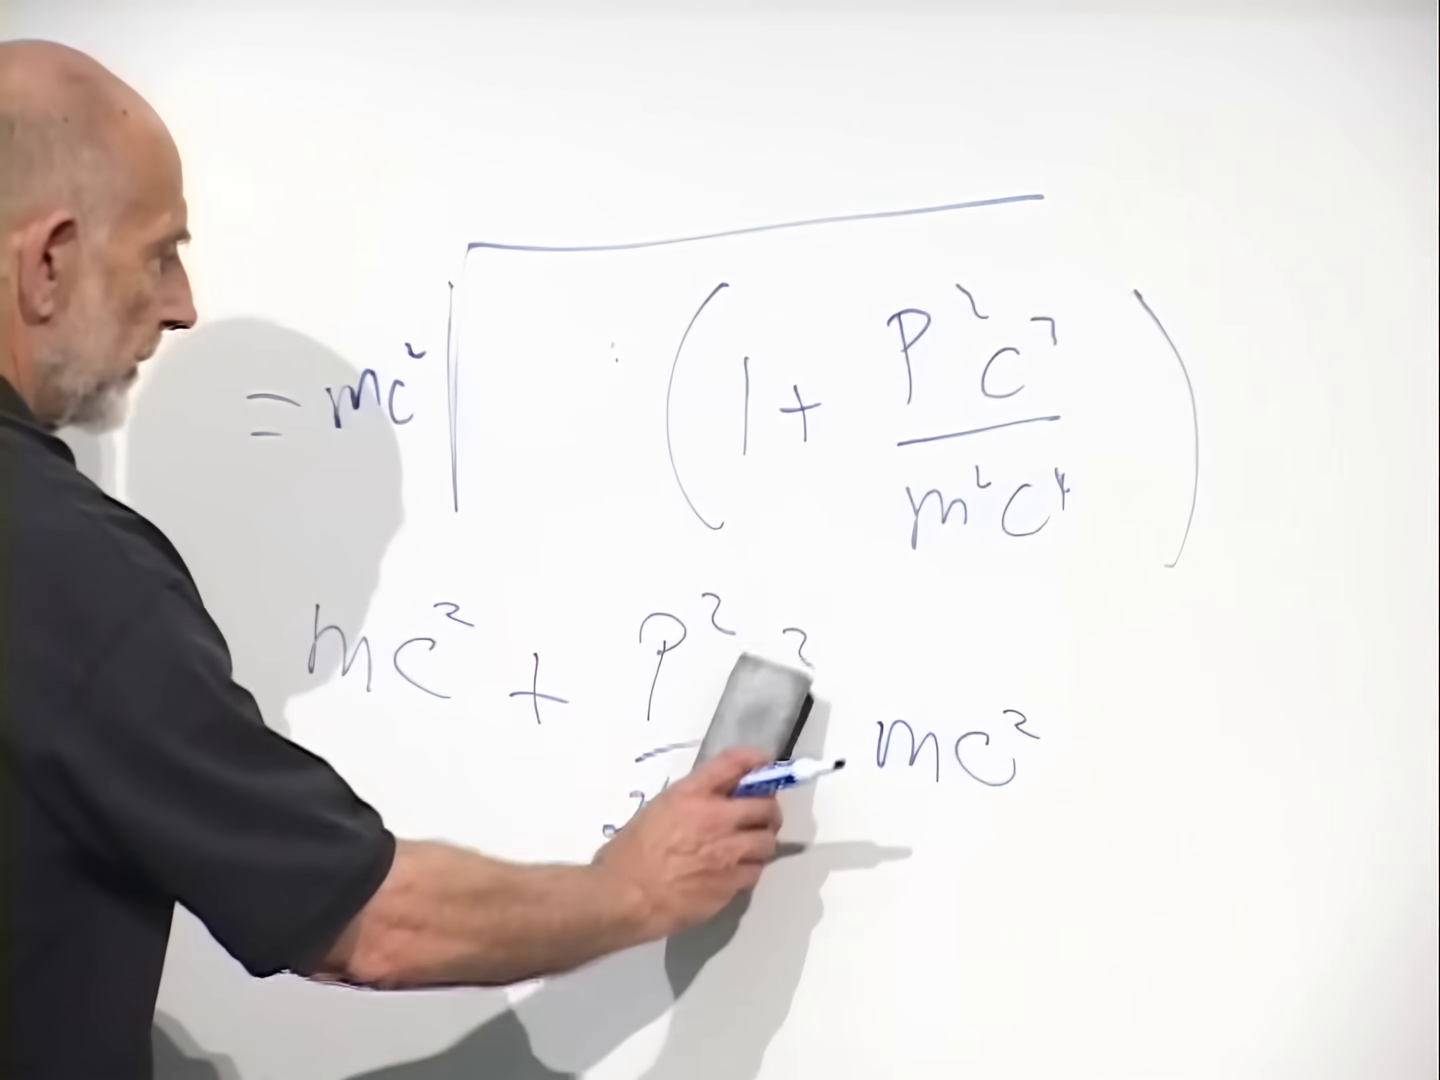
\includegraphics[width=0.76\textwidth]{lecture_01_figure_06.png}
  \caption{静止エネルギーとおなじみの非相対論的運動項を回復する小運動量展開。}
  \lectureframe{00:41:30}
  \label{fig:l01-low-momentum-board}
\end{figure}

この近似には、重心がゆっくり動くだけでは不十分である。箱がゆっくり漂いながら、その中の粒子が光速近くで運動することがある。その場合、内部の力学は依然として相対論的である。通常の非相対論的極限は、選択した座標系において関連するすべての構成粒子の速度が小さいことを要求する。

もう一つ有用な極限がある。系全体を\(z\)軸に沿ってブーストし、すべての構成粒子が大きな正の縦方向運動量\(P_{zi}\)を持つようにする。最初に後方へ運動していた構成粒子も、十分に大きなブーストによって前方へ運ばれる。横方向の運動量と静止質量は固定されたままである。

\begin{equation}
  P_{zi}\gg |p_{xi}|,|p_{yi}|,m_i,
  \qquad
  p_{\perp i}^2=p_{xi}^2+p_{yi}^2,
\end{equation}

ここでこれ以降\(c=1\)とする。大きな\(P_{zi}\)に対する展開を行うと次を得る。

\begin{align}
  E_i
  &=\sqrt{P_{zi}^2+p_{\perp i}^2+m_i^2}
  \notag\\
  &=P_{zi}\sqrt{1+\frac{p_{\perp i}^2+m_i^2}{P_{zi}^2}}
  \notag\\
  &\simeq P_{zi}
  +\frac{p_{\perp i}^2+m_i^2}{2P_{zi}}.
  \label{eq:l01-large-pz-one-particle}
\end{align}

\begin{figure}[H]
  \centering
  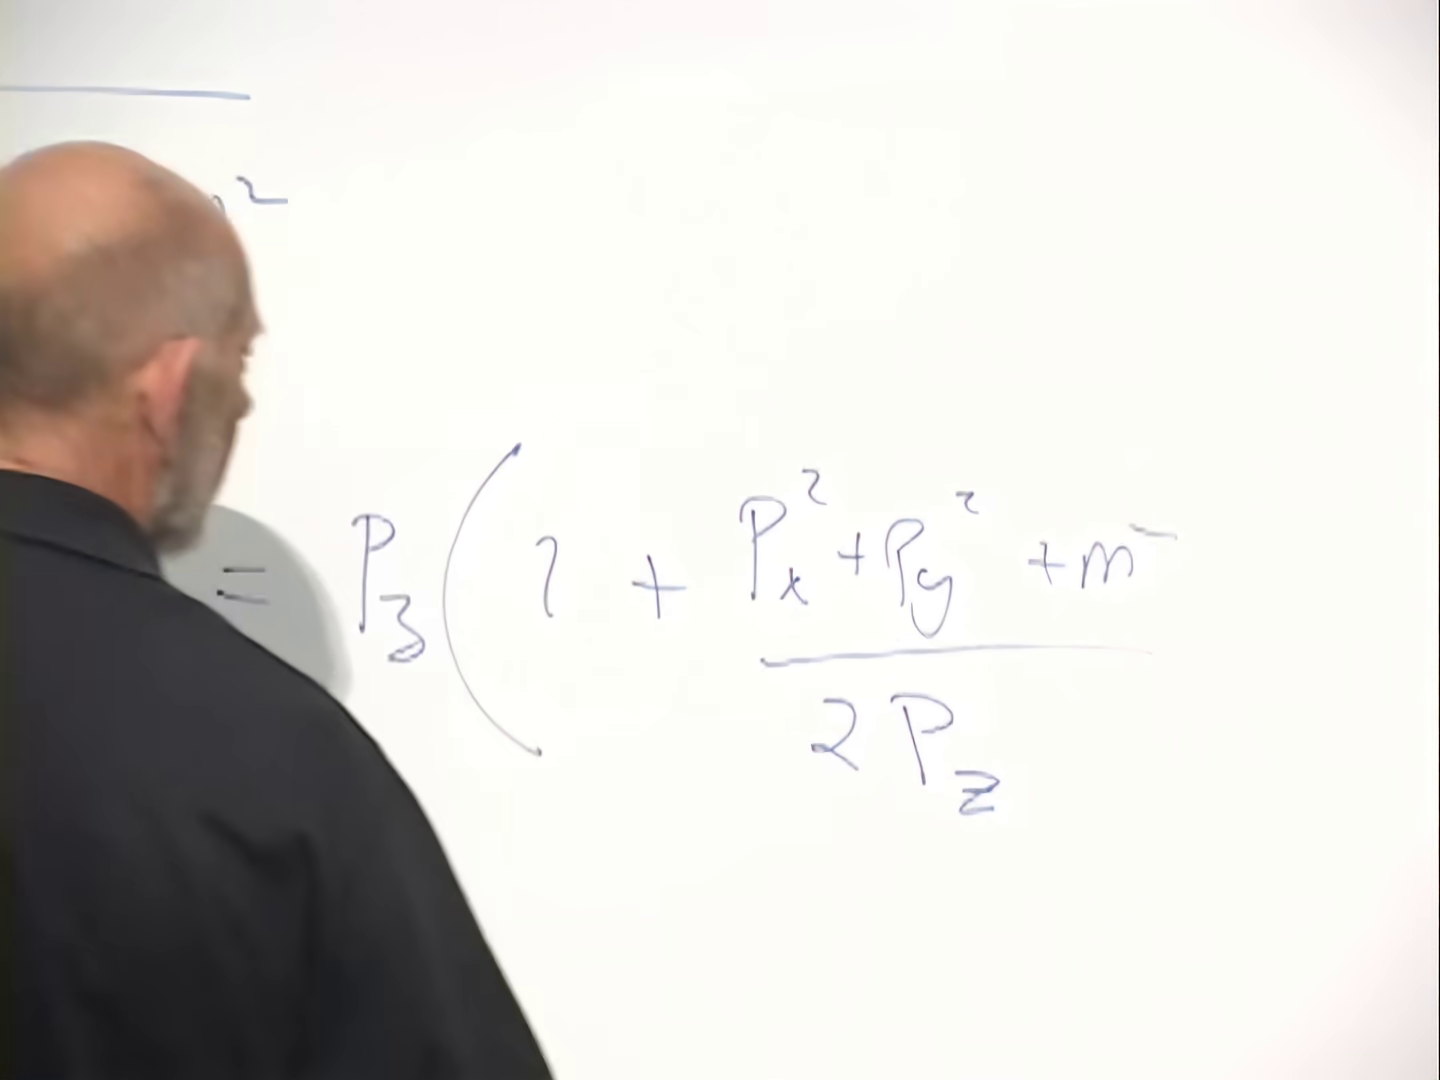
\includegraphics[width=0.76\textwidth]{lecture_01_figure_07.png}
  \caption{大きな\(P_z\)に対する平方根の展開。横方向運動量と質量を小さな量として保持している。}
  \lectureframe{00:46:45}
  \label{fig:l01-large-pz-board}
\end{figure}

多数の構成粒子に対しては、

\begin{equation}
  E\simeq
  \sum_i P_{zi}
  +\sum_i\frac{p_{\perp i}^2}{2P_{zi}}
  +\sum_i\frac{m_i^2}{2P_{zi}}.
  \label{eq:l01-large-pz-sum}
\end{equation}

第一項は保存する全縦方向運動量である。それは巨大であるが、同時に固定された加法的寄与でもある。それを保つか差し引くかはエネルギーの差を変えない。ちょうど、他の保存数をハミルトニアンに加えても運動方程式が変わらないのと同じである。したがって力学部分は

\begin{equation}
  \begin{aligned}
    H_{\perp}=E-P_z
    &\simeq
    \sum_i\left(
      \frac{p_{\perp i}^2}{2P_{zi}}
      +\frac{m_i^2}{2P_{zi}}
    \right),\\
    P_z&=\sum_iP_{zi}.
  \end{aligned}
  \label{eq:l01-transverse-hamiltonian}
\end{equation}

\begin{figure}[H]
  \centering
  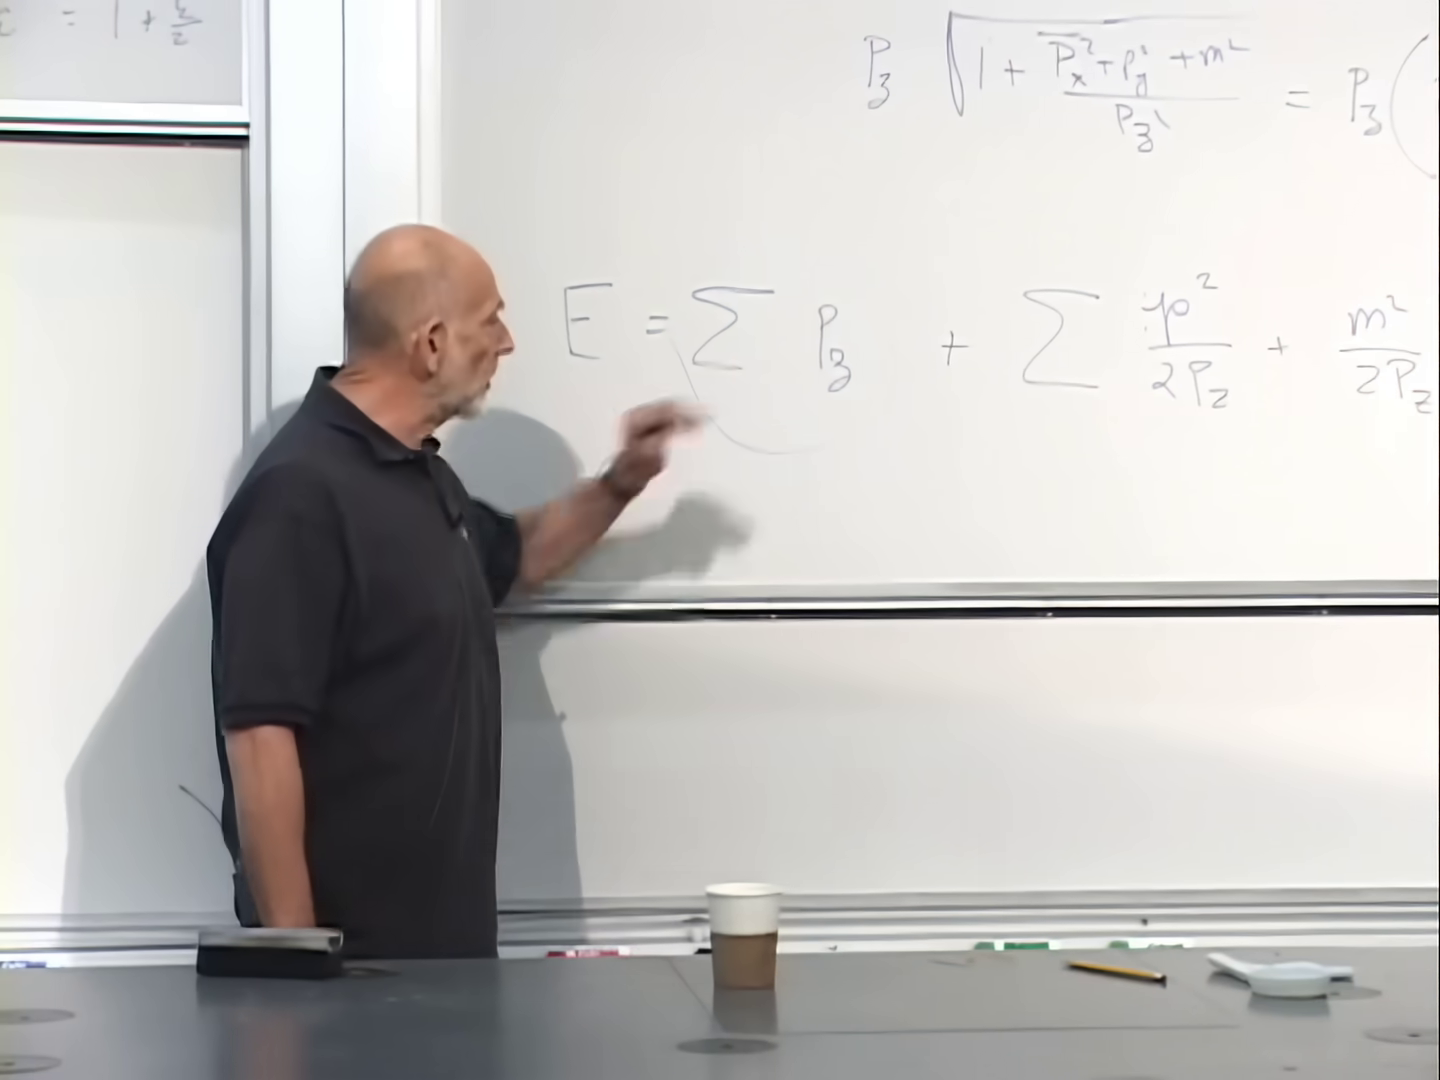
\includegraphics[width=0.78\textwidth]{lecture_01_figure_08.png}
  \caption{保存する縦方向運動量、横方向運動エネルギー、質量に依存する内部項への多粒子分解。}
  \lectureframe{00:49:16}
  \label{fig:l01-energy-sum-board}
\end{figure}

\section{無限運動量枠}

先の極限は歴史的に無限運動量枠と呼ばれ、現在では通常、光円錐座標で定式化される。その意味はハミルトニアンから直接読み取ることができる。量子力学では、

\begin{equation}
  i\hbar\frac{\partial}{\partial t}\ket{\psi}=H\ket{\psi}.
  \label{eq:l01-time-evolution}
\end{equation}

\(H_{\perp}\)のすべての非自明な項は\(1/P_z\)としてスケールする。ブーストが大きくなるにつれて、エネルギー分裂は縮小し、変化はよりゆっくり起こる。これは時間の遅れである。放射性系は強くブーストされるとよりゆっくり崩壊するように見える。比例してより長い時間観測することで補償できる。この減速は力学を除去するものではない。それらの時計を再スケールするのである。

\begin{figure}[H]
  \centering
  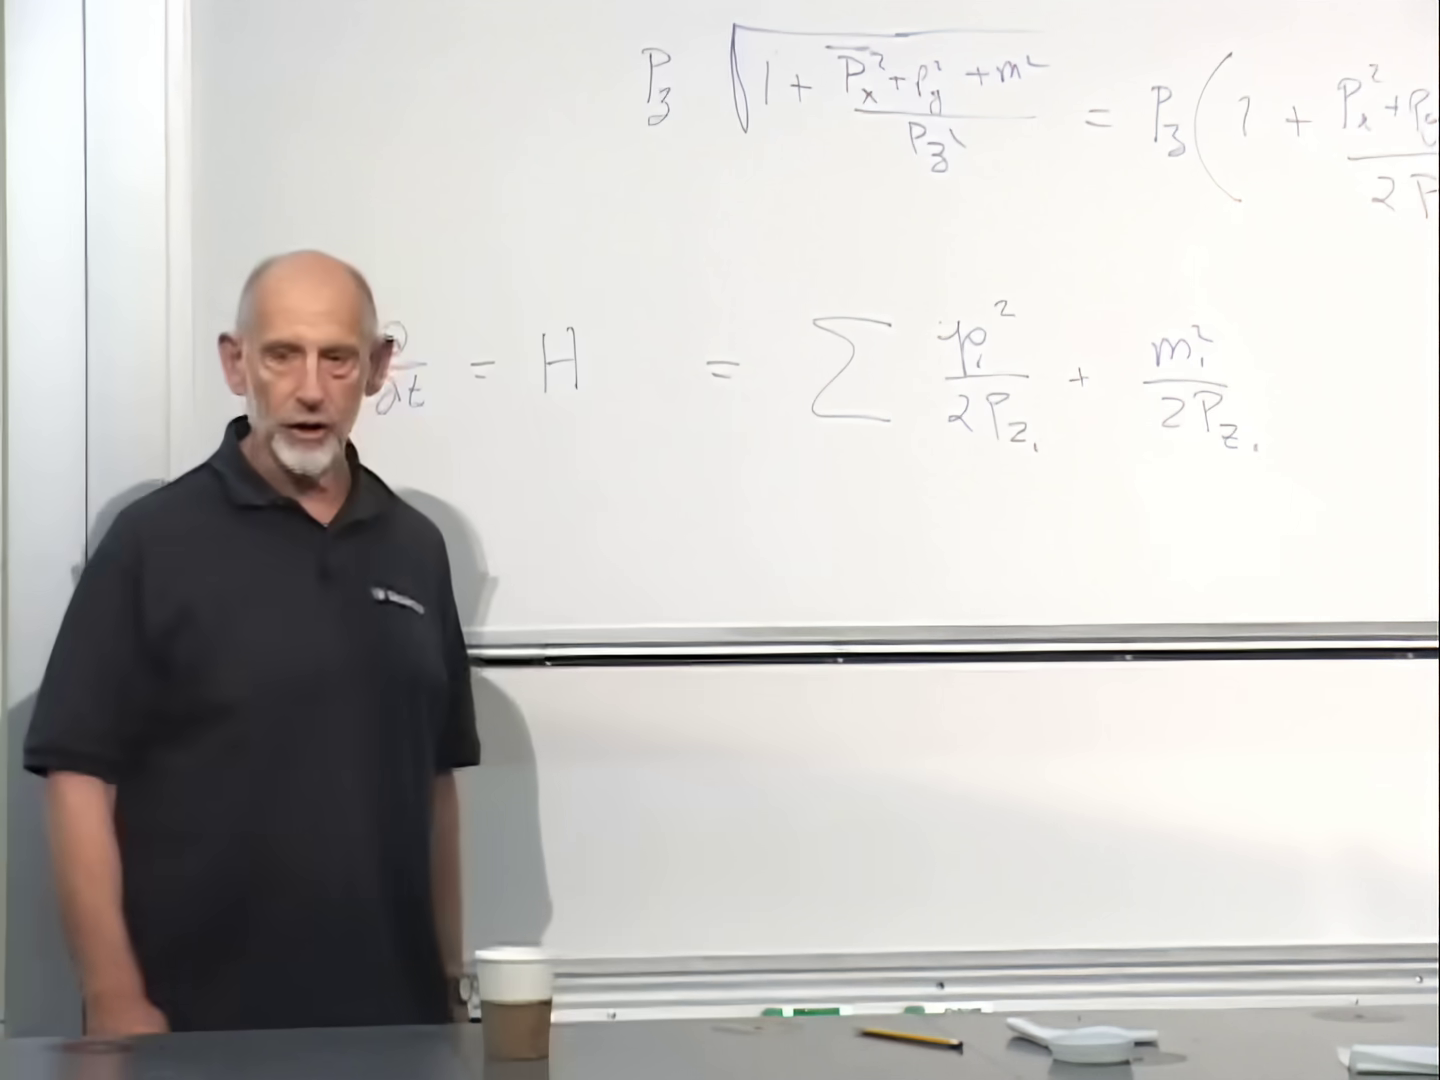
\includegraphics[width=0.78\textwidth]{lecture_01_figure_09.png}
  \caption{黒板は、換算されたエネルギーを、ブーストされた系の減速した時間発展を生成するハミルトニアンと同定している。}
  \lectureframe{00:52:57}
  \label{fig:l01-hamiltonian-board}
\end{figure}

横方向の項はまさに非相対論的な形 \(p^2/(2m)\) をしているが、質量の役割を果たすのは \(P_z\) である。これは物理的に妥当である。縦方向の運動量が大きいほど粒子を横にそらすのは難しくなるので、横方向の慣性として働く。項 \(m_i^2/(2P_{zi})\) は二次元の運動状態に依存しないため、内部エネルギーすなわち束縛エネルギーの役割を果たす。三次元空間における相対論的運動が、ブーストに垂直な二次元における非相対論的に見える運動になったのである。

これが、相対論的な弦に対して初等的な質量とばねのモデルを用いるために必要な許可である。このモデルは、弦がその静止系で遅いと装っているのではない。横方向の力学が要求される非相対論的構造をもつような系を用いているのである。

\section{ビーズとばねで作られた開弦}

開弦、すなわち二つの端点をもつ弦を考える。後にそれらの端点に何かが取り付けられるかもしれないが、ここで関心があるのは弦そのものである。横方向の位置 \(\bm X_i(t)=(X_i(t),Y_i(t))\) にあるビーズを同一のばねでつないだものによって近似する。離散的なハミルトニアンは

\begin{equation}
  H_N=\sum_{i=1}^{N}
  \left[
    \frac{\mu_N}{2}\dot{\bm X}_i^{\,2}
    +\frac{k_N}{2}
      \left(\bm X_{i+1}-\bm X_i\right)^2
  \right].
  \label{eq:l01-discrete-string}
\end{equation}

運動項だけではビーズは飛び散ってしまう。最近接のフックの項がそれらを弦にしているのである。

\begin{figure}[H]
  \centering
  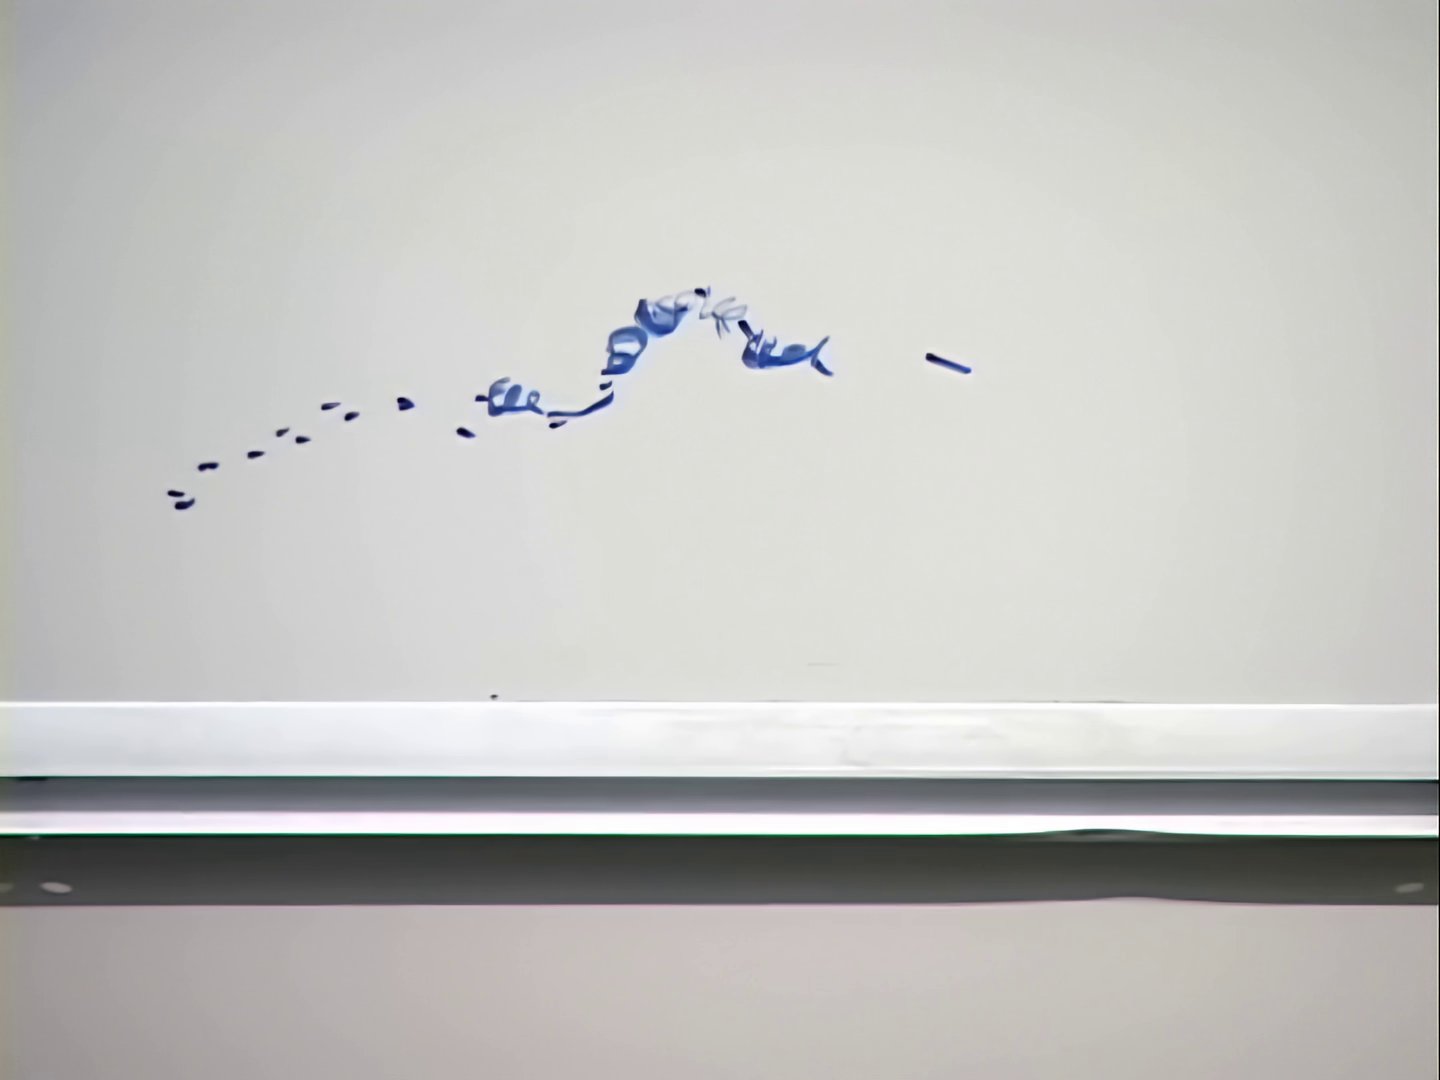
\includegraphics[width=0.75\textwidth]{lecture_01_figure_10.png}
  \caption{二つの横方向座標をもつ開弦に対する最初のビーズとばねのスケッチ。}
  \lectureframe{01:00:30}
  \label{fig:l01-bead-chain-board}
\end{figure}

\begin{figure}[H]
  \centering
  \begin{tikzpicture}[>=Latex]
    \foreach \x in {0,...,8} {
      \fill[blue!65!black] ({0.85*\x},0) circle (0.09);
    }
    \foreach \x in {0,...,7} {
      \draw[decorate,decoration={zigzag,segment length=4pt,amplitude=2pt}]
        ({0.85*\x+0.10},0) -- ({0.85*\x+0.75},0);
    }
    \draw[->] (3.4,0.15) -- (3.4,1.25) node[above] {$\bm X_i(t)$};
    \draw[<->] (0,-0.65) -- (6.8,-0.65)
      node[midway,below] {$0\leq\sigma\leq\pi$};
  \end{tikzpicture}
  \caption{開弦に対する離散的正則化。ビーズの質量とばね定数は、連続極限をとる前に間隔に応じてスケールする。}
  \label{fig:l01-bead-chain-redraw}
\end{figure}

\begin{figure}[H]
  \centering
  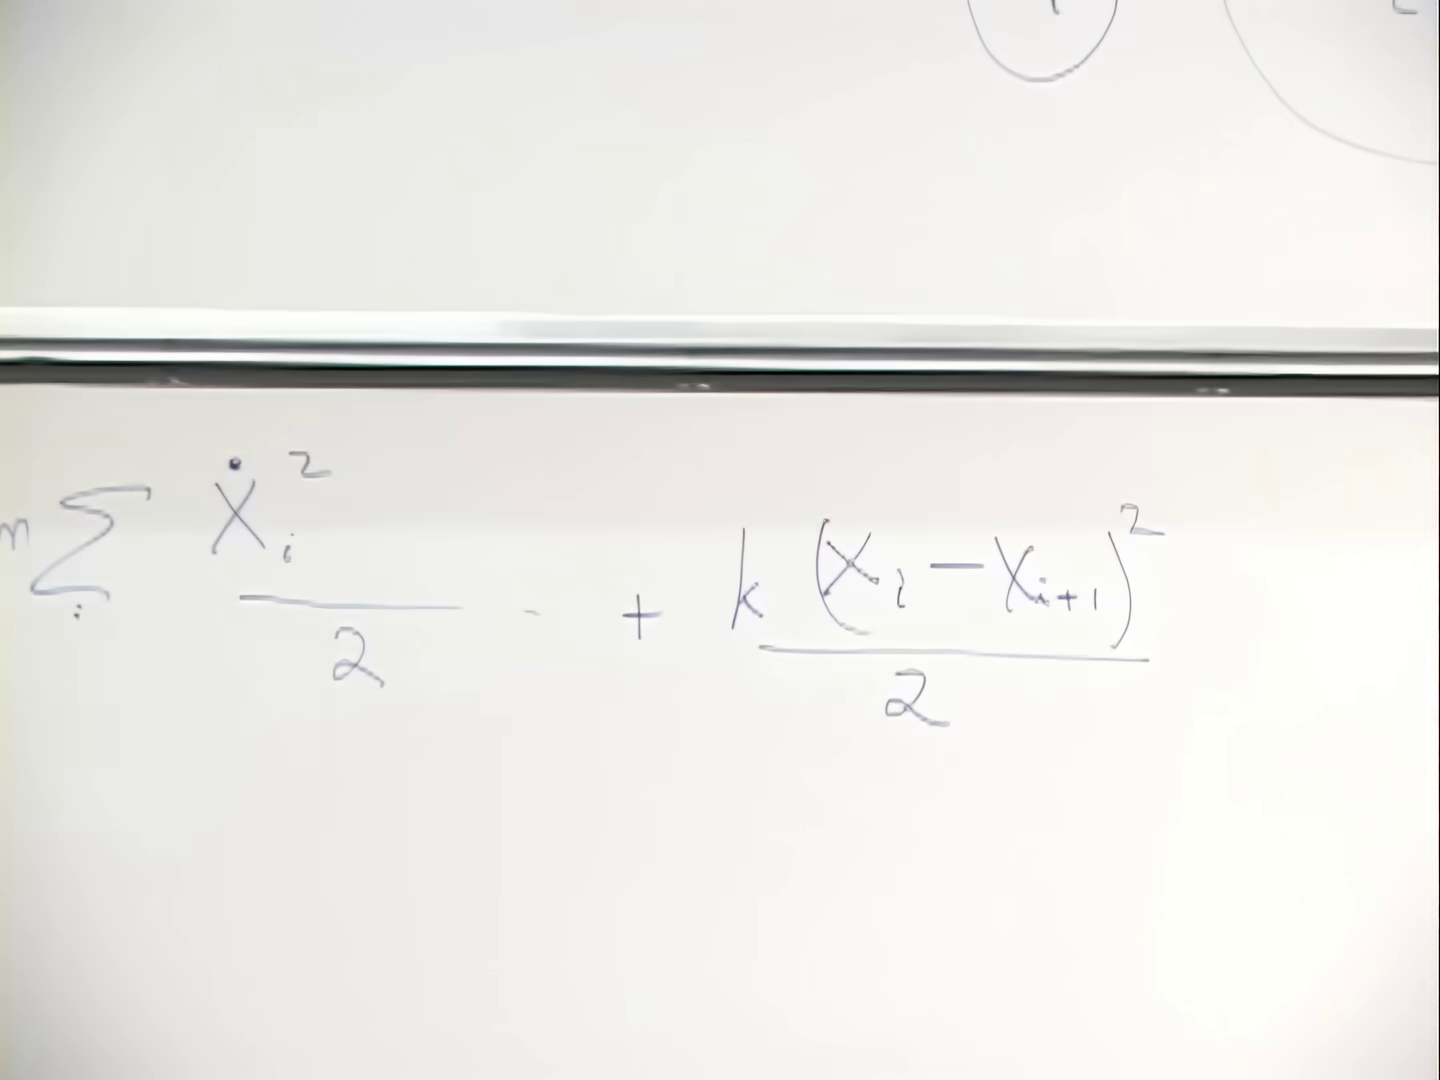
\includegraphics[width=0.78\textwidth]{lecture_01_figure_11.png}
  \caption{連続極限の前にまとめて書かれた離散的な運動項とフックの項。}
  \lectureframe{01:01:30}
  \label{fig:l01-discrete-energy-board}
\end{figure}

ビーズの数が増えるにつれて、各ビーズの質量 \(\mu_N\) は弦全体が有限の慣性を保つようにゼロに近づかなければならない。同時にばね定数 \(k_N\) は大きくなければならない。長いゴムの帯は同じ材料の微小な断片よりも一定量だけ伸ばすのが容易である。したがって、連続体の材料が同じままでいるためには、より近くに寄せられた隣接点はより剛くつながれなければならない。

弦に沿った座標 \(\sigma\) を導入する。その数値範囲は約束事である。

\begin{equation}
  0\leq\sigma\leq\pi
\end{equation}

と選ぶと、後に閉弦を \(0\) から \(2\pi\) までパラメータ付けできるので便利である。和は積分になり、最近接差分は微分になる。

\begin{equation}
  \sum_i\longrightarrow\int_0^\pi d\sigma,
  \qquad
  \bm X_{i+1}-\bm X_i
  \longrightarrow
  \partial_\sigma\bm X.
  \label{eq:l01-continuum-replacements}
\end{equation}

\(t\)、\(\sigma\)、\(\bm X\) の規格化に間隔に依存する定数を吸収した後、連続的なハミルトニアンは次の形をとる。

\begin{equation}
  H_{\mathrm{string}}=
  \frac12\int_0^\pi d\sigma
  \left[
    \left(\partial_t\bm X\right)^2
    +\left(\partial_\sigma\bm X\right)^2
  \right].
  \label{eq:l01-continuum-hamiltonian}
\end{equation}

\begin{figure}[H]
  \centering
  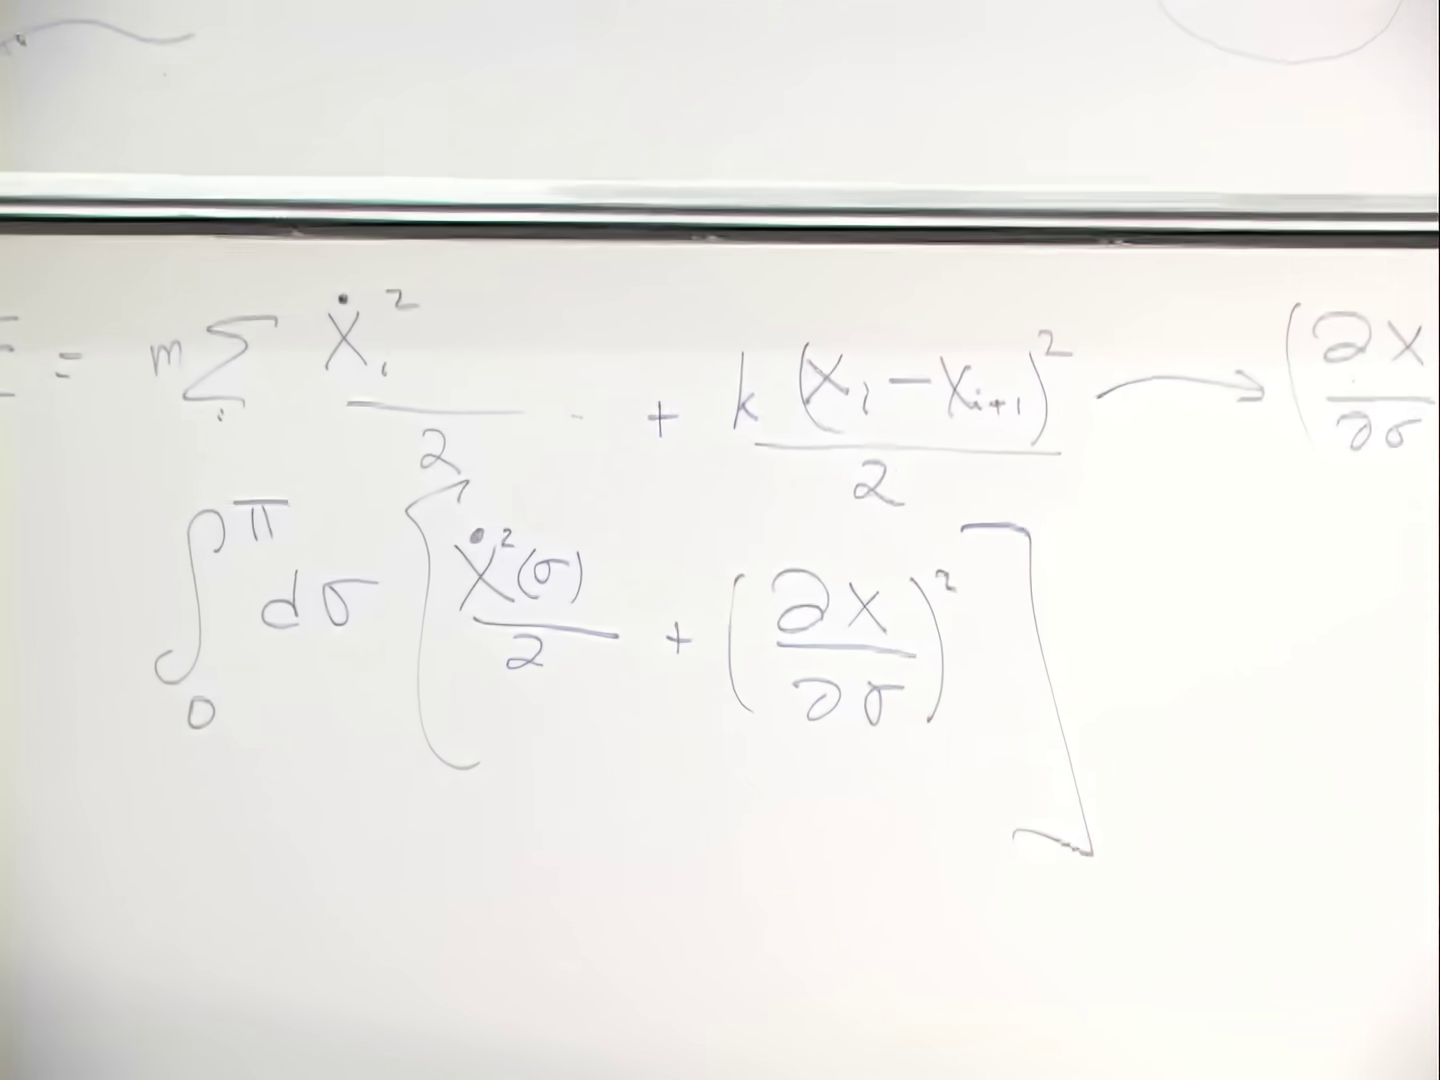
\includegraphics[width=0.78\textwidth]{lecture_01_figure_12.png}
  \caption{ビーズの和から \(\int_0^\pi d\sigma\) への板書の過程。最近接差分は \(\partial_\sigma\bm X\) に置き換えられている。}
  \lectureframe{01:05:00}
  \label{fig:l01-continuum-board}
\end{figure}

第一項は二つの横方向の運動エネルギーである。第二項は弦に沿った伸びを測る。これがハミルトニアンであるため、両方の項はプラス符号をもつ。ラグランジアンではポテンシャル項はマイナス符号で入るであろう。正確な係数は約束事に依存し、この段階では固定されていない。運動プラス伸びの構造が重要になるのである。

重心運動を相対運動から分離する。すべての点を同じ量だけ平行移動することは粒子全体を動かす。振動、曲げ、相対的な伸びは内部運動である。陽子、原子、その他の複合的な物体は、その構成要素が内部的に運動していても粒子と呼ぶことができる。弦もその点では同じである。

\section{なぜハミルトニアンが質量の二乗を測るのか}

ゆっくり動く物体では、静止エネルギーはその質量に比例する。しかし無限運動量の記述では、内部からの寄与は \(M^2/(2P_z)\) として現れる。共通の縦方向運動量とそれに伴う時間の再スケーリングが固定されれば、内部の弦のハミルトニアンは物体全体の不変質量の二乗に比例する。

\begin{equation}
  H_{\mathrm{int}}\propto M^2.
  \label{eq:l01-hint-mass-squared}
\end{equation}

\editorialnote{より明示的には、光円錐の運動学は \(M^2=2P^+P^- - \bm P_\perp^2\) の形の不変な関係を与える。重心横方向系で \(P^+\) を固定すると、光円錐ハミルトニアン \(P^-\) はしたがって \(M^2\) に比例する。講義ではこれらの規格化の詳細を省き、議論に必要な比例関係を保っている。}

\begin{figure}[H]
  \centering
  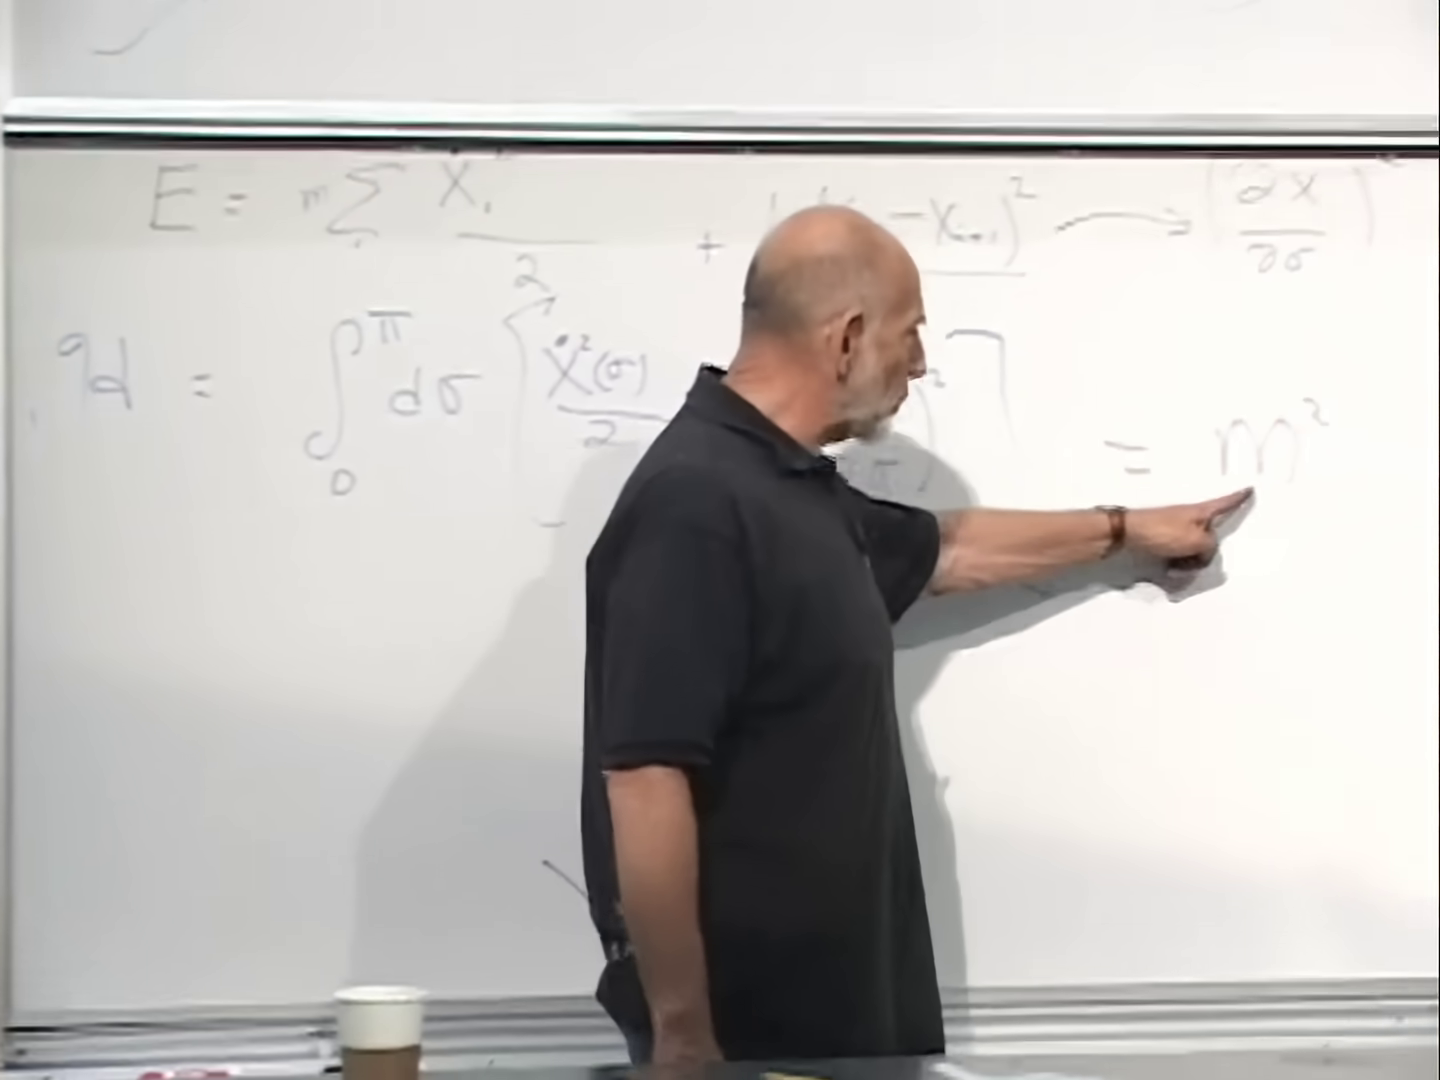
\includegraphics[width=0.76\textwidth]{lecture_01_figure_13.png}
  \caption{板書は内部の弦のエネルギーを弦状態全体の質量の二乗と同一視している。}
  \lectureframe{01:10:30}
  \label{fig:l01-mass-squared-board}
\end{figure}

振動する弦は結合した振動子の集まりである。その完全な量子化は後回しにするが、重要なスペクトルの事実はすでに見えている。調和振動子のエネルギーは離散的な段階で増大する。それらの内部エネルギーは\(M^2\)に寄与するので、弦の励起は自然に質量の二乗に離散的な段階を生じる。これが冒頭でレッジェプロットが告げていた構造である。

\begin{classroomqa}
\audiencequestion{\(M\)は弦全体の質量ですか。また、その質量を二倍にすると、対応する\(M^2\)の寄与は四倍になりますか。
\lecturetimestamp{01:12:10}}
\lecturerresponse{はい。\(M\)は、振動、伸長、その他すべての内部寄与を含む、完全な弦状態の静止質量です。有効ブーストハミルトニアンは\(M^2\)に比例するので、質量が二倍の状態では、その質量の二乗の値は四倍になります。}
\end{classroomqa}

\begin{classroomqa}
\audiencequestion{静止質量がゼロである光子を、この記述はどのように含むことができるのか。\lecturetimestamp{01:12:52}}
\lecturerresponse{質量ゼロの状態は\(M=0\)に対応する。正の振動子の寄与がどのように結合してそのような状態を生じうるかは、量子化された理論にとって重要な問題であり、ここでの古典的模型によって決着するものではない。この時点では\(M\)は単に全静止質量を表しており、量子力学はまだ導入されていない。}
\end{classroomqa}

次に、動いていない弦を物理的な長さ\(L\)まで一様に伸ばす。運動項は消え、長さ\(\pi\)のパラメータ区間にわたって、

\begin{equation}
  \left|\partial_\sigma\bm X\right|\simeq\frac{L}{\pi}.
\end{equation}

したがって、

\begin{align}
  H_{\mathrm{stretch}}
  &\propto
  \int_0^\pi d\sigma
    \left(\partial_\sigma\bm X\right)^2
  \notag\\
  &\simeq
  \pi\left(\frac{L}{\pi}\right)^2
  \propto L^2.
  \label{eq:l01-hooke-l2}
\end{align}

\begin{figure}[H]
  \centering
  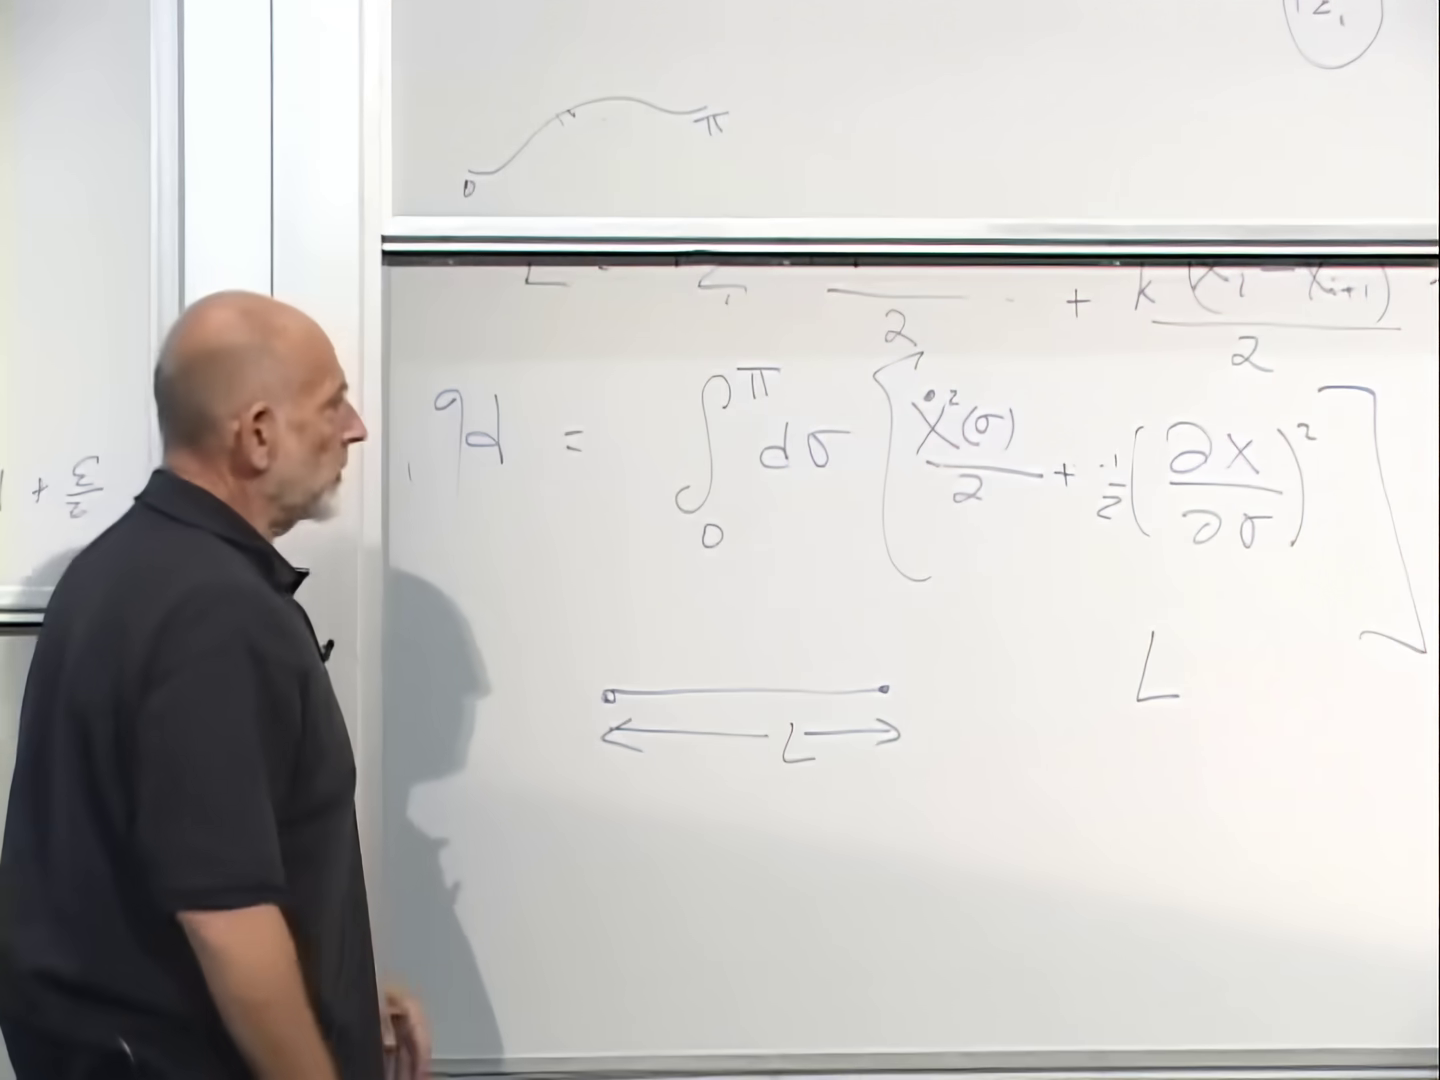
\includegraphics[width=0.76\textwidth]{lecture_01_figure_14.png}
  \caption{\(H_{\mathrm{stretch}}\propto L^2\)を推論し、したがって\(M\propto L\)を推論するために用いられた、一様に伸ばされた配置。}
  \lectureframe{01:15:30}
  \label{fig:l01-length-relation-board}
\end{figure}

これは有効な横方向の力学におけるフックの法則の振る舞いである。しかし左辺の量は\(M\)ではなく\(M^2\)に比例する。したがって次のことが従う。

\begin{equation}
  M^2\propto L^2,
  \qquad
  M\propto L.
  \label{eq:l01-mass-length}
\end{equation}

静止系ではエネルギーは\(c=1\)の単位で\(E_{\mathrm{rest}}=M\)である。比例定数を弦の張力\(T\)と書くと、

\begin{equation}
  E_{\mathrm{rest}}=TL.
  \label{eq:l01-string-tension}
\end{equation}

この結果はフラックスチューブの描像と一致する。一様な電場または磁場は一様なエネルギー密度を運ぶ。そのフラックスが一定の断面積をもつチューブに閉じ込められているなら、長さが一単位増えるごとに同じ量のエネルギーが加わる。等価に、新たに開いた隙間を新しい自由度が埋めていく構成要素描像では、単位長さあたりのエネルギーは一定である。弦の張力とは、その単位長さあたりのエネルギーである。

この結論は間接的である。相対論的な速度まで駆動された任意のゴムバンドが自動的に\(E=TL\)を獲得する、と主張しているのではない。議論は大きなブーストから従う横方向の非相対論的記述から始まり、その内部エネルギーを\(M^2\)と同定し、その後に初めて結果を静止系のエネルギーへと翻訳する。

\section{二つの系における同じ対象}

\(M\)と\(M^2\)の区別は失われやすいので、二つの展開を並べて置く価値がある。\(c=1\)として、

\begin{align}
  E&=\sqrt{p^2+M^2}
  \simeq M+\frac{p^2}{2M},
  &&p\ll M,
  \label{eq:l01-rest-expansion-again}\\
  E&=\sqrt{P_z^2+M^2}
  \simeq P_z+\frac{M^2}{2P_z},
  &&P_z\gg M.
  \label{eq:l01-boost-expansion-again}
\end{align}

\begin{figure}[H]
  \centering
  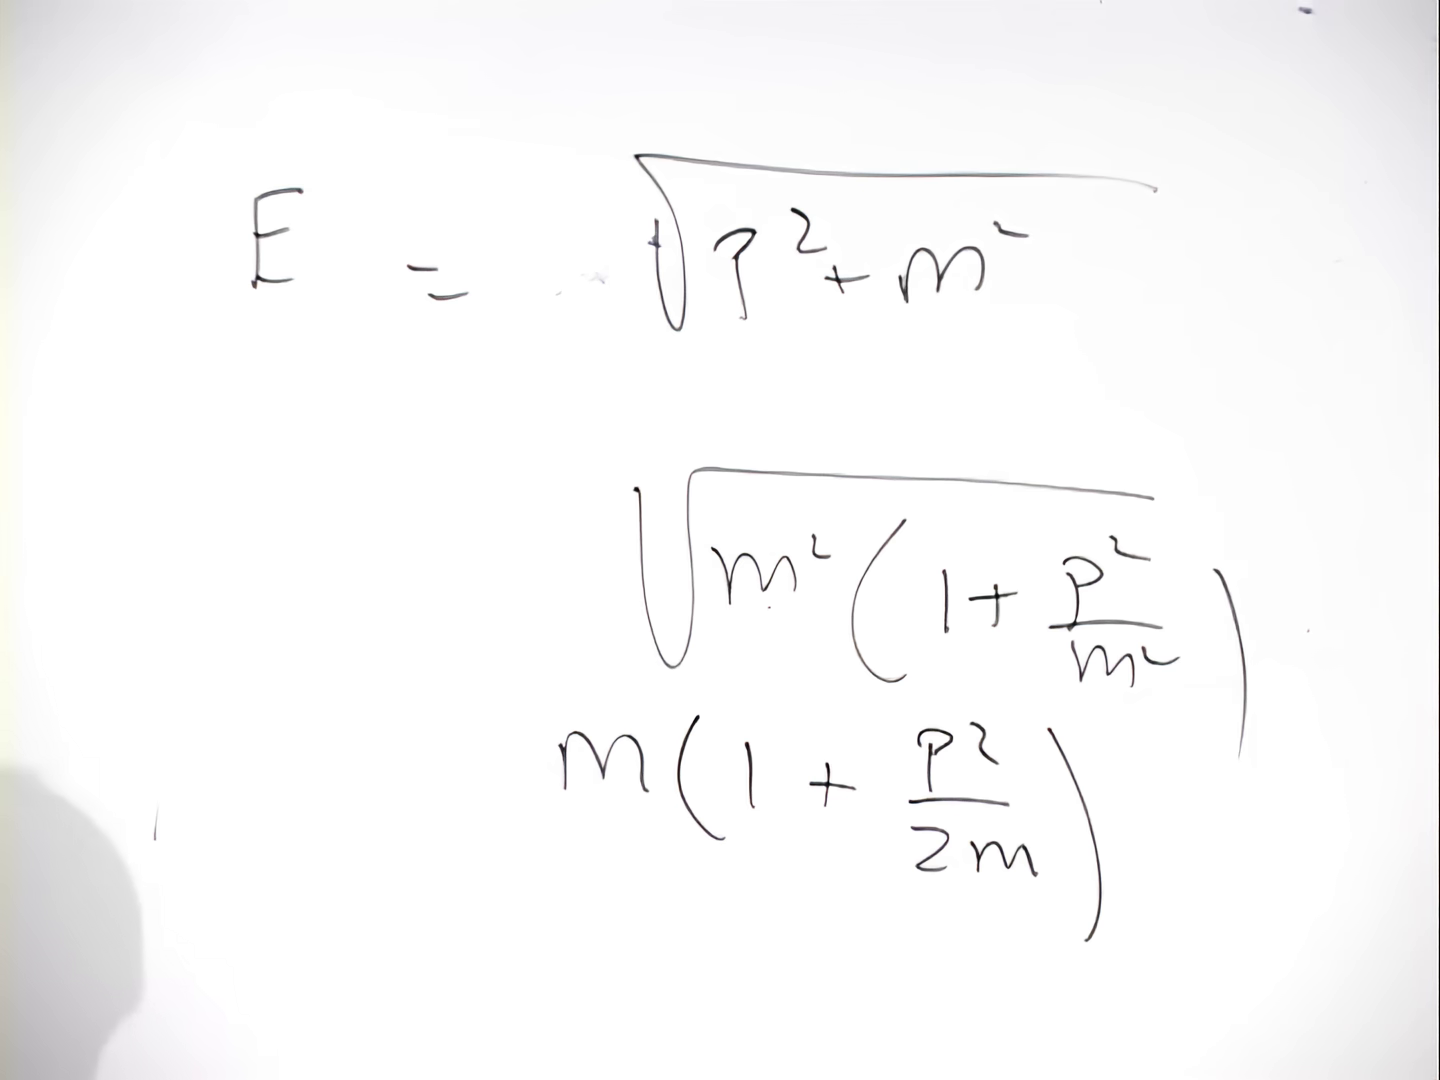
\includegraphics[width=0.74\textwidth]{lecture_01_figure_15.png}
  \caption{区切りの後に繰り返される小運動量展開。ここで内部静止エネルギーは\(M\)と読まれる。}
  \lectureframe{01:28:00}
  \label{fig:l01-rest-expansion-board-again}
\end{figure}

\begin{figure}[H]
  \centering
  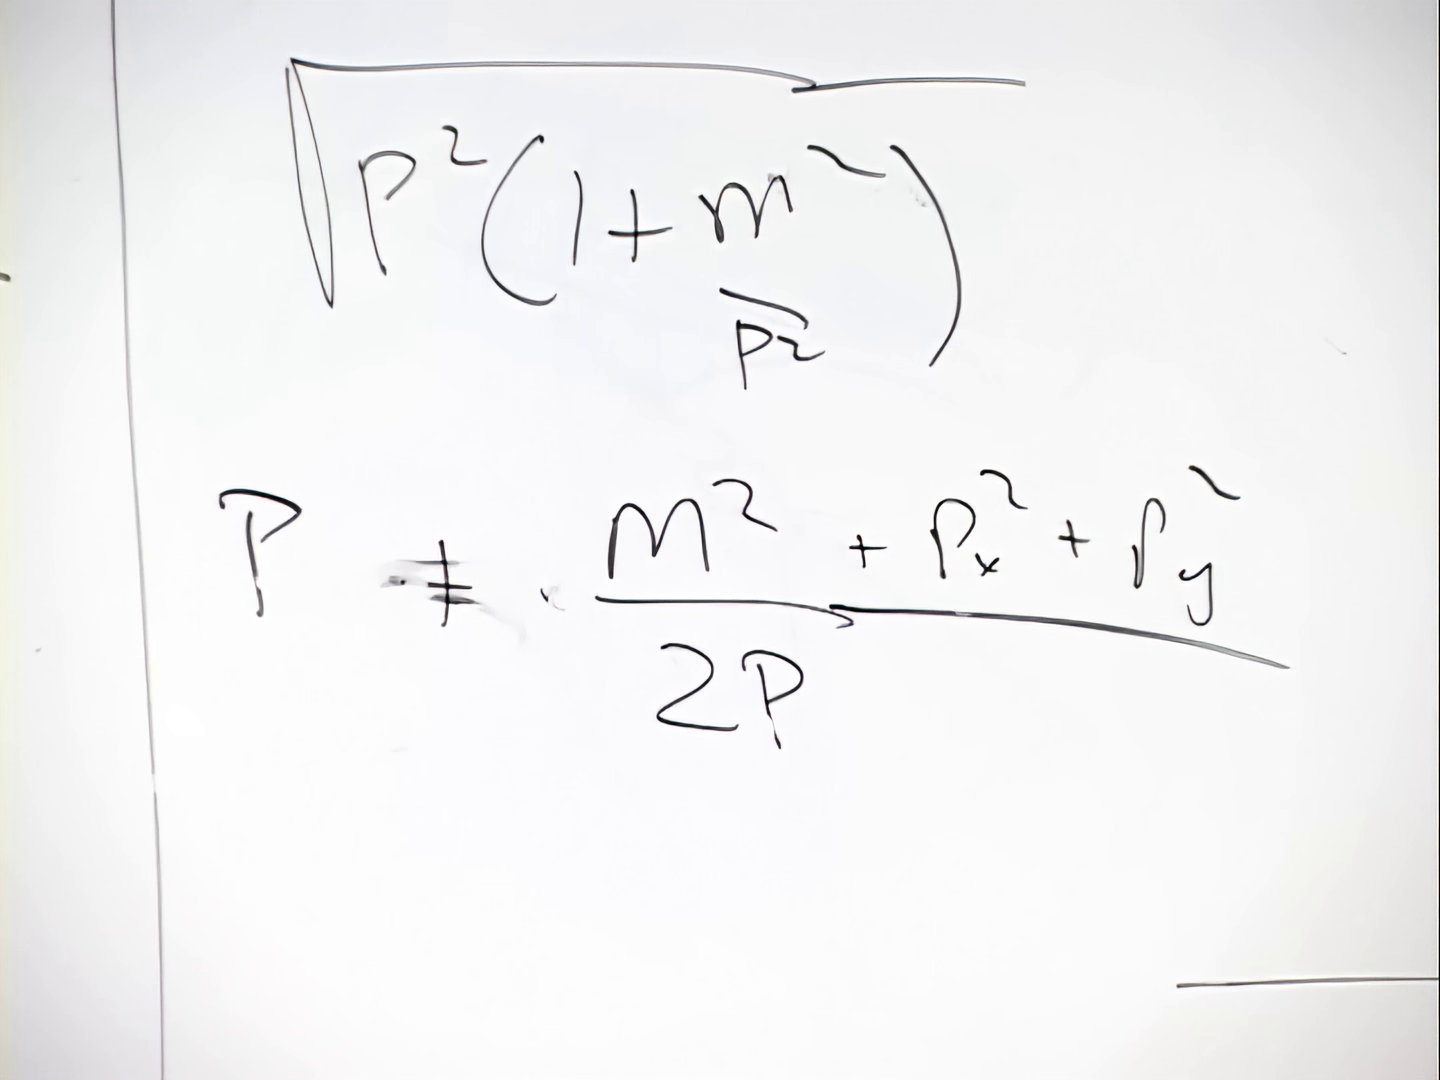
\includegraphics[width=0.74\textwidth]{lecture_01_figure_16.png}
  \caption{相補的な大運動量展開。ここで残りのエネルギーは\(M^2/(2P_z)\)に比例する。}
  \lectureframe{01:31:00}
  \label{fig:l01-boost-expansion-board-again}
\end{figure}

第一の展開は静止エネルギーを質量と同定し、通常の慣性を\(M\)と同定する。第二の展開では、保存される\(P_z\)の項が取り除かれ、横方向の慣性は\(P_z\)であり、内部エネルギーは\(M^2/(2P_z)\)で表される。質量はどちらの系でも弦の長さに比例したままである。変わるのは、質量のどの関数が残りのハミルトニアンとして現れるかである。

\begin{classroomqa}
\audiencequestion{ローレンツブーストは物理を変えるはずがない。なぜブーストされた弦は異なるエネルギー法則に従うように見えるのか。
\lecturetimestamp{01:25:35}}
\lecturerresponse{異なる物理に従っているのではない。どちらの記述でも\(M\propto L\)であり、\(M^2\propto L^2\)である。静止系では関係するエネルギーは\(M\)であり、大きなブーストの後では保存される\(P_z\)が分離され、残りのハミルトニアンは\(M^2\)に比例する。ブーストが変えるのは有用な記述であり、不変質量--長さの関係ではない。}
\end{classroomqa}

\section{閉じ込めの超伝導模型}

超伝導体は磁場をそのバルクから排除する。物質が超伝導状態になる前に、十分に狭いチャネルを通して磁束が捕獲されると、その磁束は横方向に広がることができず、管の中に閉じ込められたままになる。有用な思考実験は、常伝導状態の試料に細い穴を開け、そこに長い棒磁石を挿入し、試料を冷却してから磁石を引き抜くというものである。この構成は実際の実験室の手順というよりも模式的なものである。その目的は、磁場の強さとエネルギー密度がその長さに沿ってほぼ一様である磁束線を孤立させることにある。

\begin{figure}[H]
  \centering
  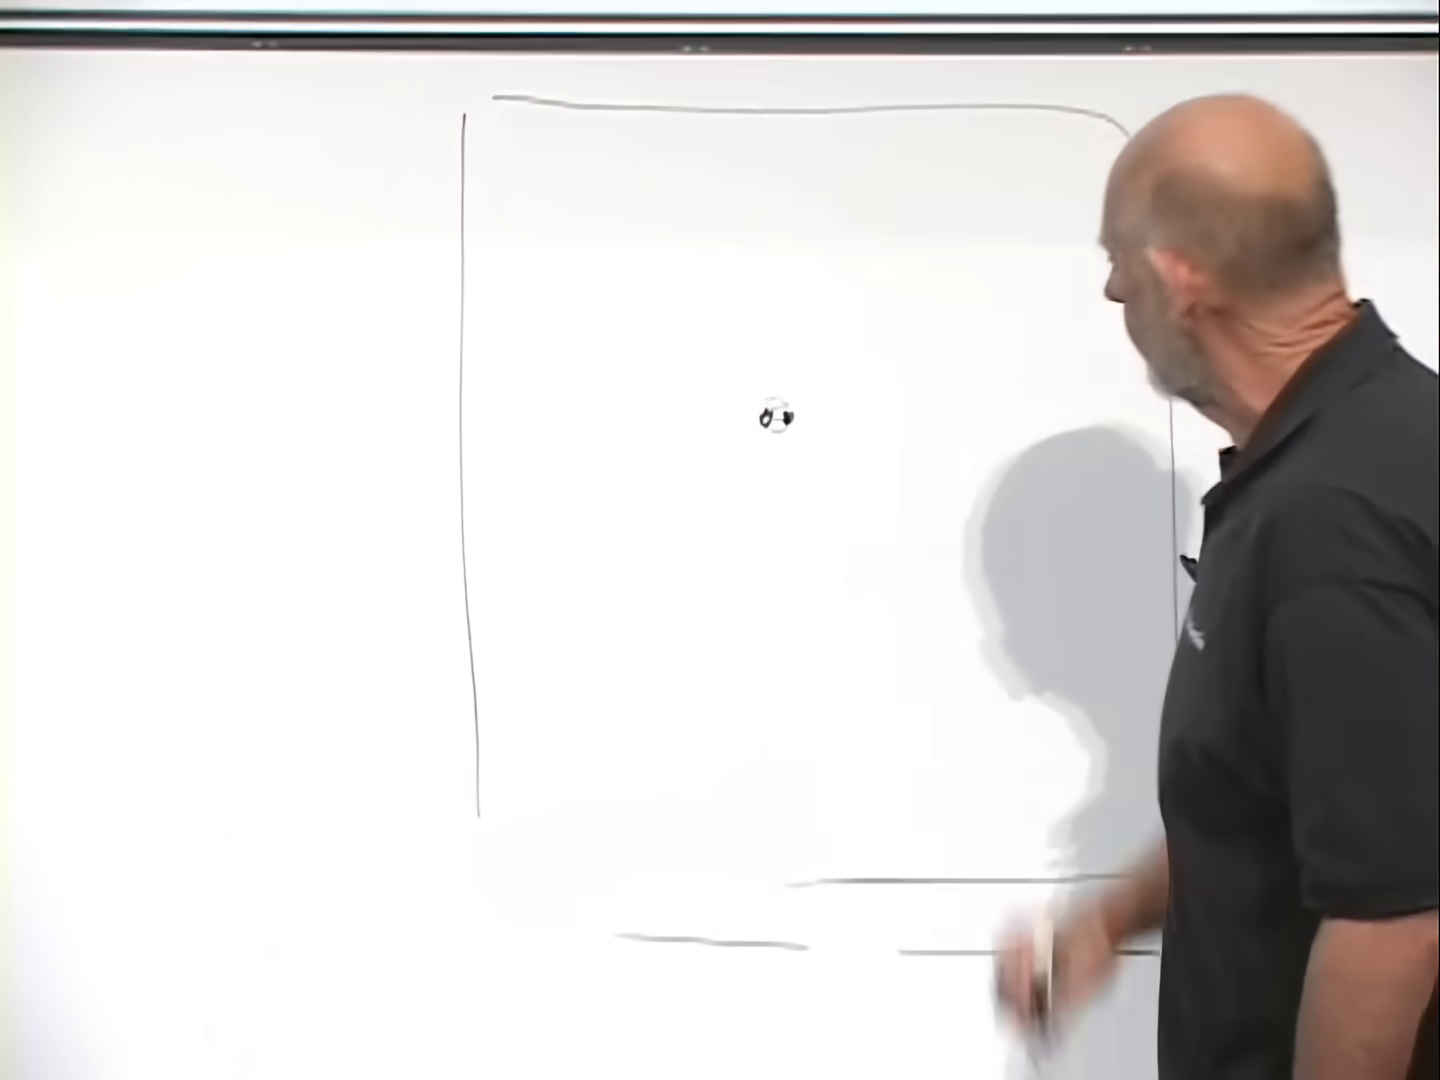
\includegraphics[width=0.76\textwidth]{lecture_01_figure_17.png}
  \caption{超伝導磁束線の構成と、対応するモノポール--アンチモノポール閉じ込めの描像。}
  \lectureframe{01:35:30}
  \label{fig:l01-superconductor-board}
\end{figure}

さらなる思考実験として、磁気モノポールとアンチモノポールを超伝導媒質中に置いて引き離すことができたとしよう。それらの間の磁束は管に絞り込まれるであろう。管の単位長さが同じエネルギーを運ぶので、

\begin{equation}
  V(R)=T_{\mathrm{flux}}R.
  \label{eq:l01-linear-confinement}
\end{equation}

力\(F=-dV/dR\)は一定の大きさをもつ。対を引き離すことはますます高くつくようになるので、対は閉じ込められる。これがハドロン中のクォークに求められる振る舞いである。

\begin{figure}[H]
  \centering
  \begin{tikzpicture}[>=Latex]
    \fill[blue!8,rounded corners=5pt] (-4,-1.35) rectangle (4,1.35);
    \node[blue!55!black] at (0,1.65) {superconducting medium};
    \fill[red!75!black] (-2.8,0) circle (0.17);
    \fill[blue!70!black] (2.8,0) circle (0.17);
    \node[below] at (-2.8,-0.22) {monopole};
    \node[below] at (2.8,-0.22) {antimonopole};
    \fill[orange!18,rounded corners=7pt] (-2.65,-0.42) rectangle (2.65,0.42);
    \draw[orange!85!black,thick,rounded corners=7pt]
      (-2.65,-0.42) rectangle (2.65,0.42);
    \foreach \y in {-0.22,0,0.22}
      \draw[->,orange!85!black] (-2.55,\y) -- (2.55,\y);
    \draw[<->] (-2.8,-1.00) -- (2.8,-1.00) node[midway,below] {$R$};
  \end{tikzpicture}
  \caption{磁束の閉じ込めは一様な管と線形ポテンシャル\(V(R)=T_{\mathrm{flux}}R\)を与える。}
  \label{fig:l01-superconductor-redraw}
\end{figure}

\begin{classroomqa}
\audiencequestion{ハドロンにおいて超伝導媒質の役割を果たすものは何か。\lecturetimestamp{01:36:57}}
\lecturerresponse{提案された類推は電気と磁気の役割を逆転させる。通常の超伝導凝縮体は電気的に荷電しており、磁束を閉じ込める。QCDの双対超伝導体描像では、クロモ磁気的な物体の凝縮体がクォークのクロモ電荷を閉じ込める。そのような物体は真空中で凝縮しているものとして表されるため、孤立した粒子としては現れない。}
\end{classroomqa}

\editorialnote{双対超伝導体による記述は影響力のある閉じ込め機構であり、ここでは講義の歴史的な言葉遣いで提示されている。これはQCD真空の物理的描像として読まれるべきであり、第一原理からの閉じ込めの完全な導出としてではない。}

\begin{classroomqa}
\audiencequestion{エネルギーが長さに比例することは、高度に相対論的にされた任意の通常の弦に対する一般的な規則か。\lecturetimestamp{01:38:10}}
\lecturerresponse{いいえ。まずその物質についての整合的な相対論的理論が必要であり、その振る舞いは詳細に依存するであろう。線形なエネルギーは、引き延ばされても密度が固定されたままである配置、あるいは横方向に広がることを妨げられた磁束に特有のものである。それを引き離すことは、固定された分子の集合の間隔を単に広げるのではなく、より多くの構成要素、あるいはより多くの一様な磁場で満たされた長さを生み出す。}
\end{classroomqa}

\section{横方向の自由度と粒子の大きさ}

光円錐構成は弦をその横座標によって直接書き表す。各横振動子に対応する、別個に自由に指定できる縦振動子は存在しない。この直接的な空間次元一つ分の削減はこの形式の注目すべき特徴の一つであるが、完全な理論はそれでもなおローレンツ不変性を満たさなければならない。

\begin{classroomqa}
\audiencequestion{\(z\)方向に沿った残りの運動はどうなるのか。\lecturetimestamp{01:40:10}}
\lecturerresponse{光円錐記述では、縦方向の運動は独立な自由度として導入されない。物理的な振動は横方向に記述され、一方で拘束条件が縦方向の情報を決定する。この経済性は、重力を及ぼす系が直接的な次元を一つ減らした記述を許すかもしれないという考えと精神において関連しているが、そのつながりはここでは導出されない。}
\end{classroomqa}

\begin{classroomqa}
\audiencequestion{レッジェプロット上で実際に知られている点はいくつあるのか。\lecturetimestamp{01:41:15}}
\lecturerresponse{正確な最大数は族に依存する。おおよその数は七つほどである。この系列は実験的に無限に続くものではない。関連する事実は、知られている点が、通常の巨視的な物質で見慣れた種類の目に見える破綻や分裂の端点を示さないということである。}
\end{classroomqa}

ハドロンの現象論が歴史的な動機を与えたが、数学的な弦理論はハドロンをあらゆる細部まで再現することを要求されない。ひとたび形式が構築されれば、それが実際に何を記述するのかが問われる。その質量ゼロのスピン2状態やその他の性質は、より自然に重力を指し示す。

ハドロンと電子の間の見かけの対比は、剛体回転のエネルギーによって定量化できる。

\begin{equation}
  E_{\mathrm{rot}}=\frac{J^2}{2I},
  \qquad
  I\sim MR^2.
  \label{eq:l01-rotational-energy}
\end{equation}

角運動量は量子化される。\(J^2\)を模式的に\(\hbar^2 n^2\)と書くと、最初の回転の段階は程度である

\begin{equation}
  \Delta E_{0\to1}\sim\frac{\hbar^2}{2I}.
  \label{eq:l01-first-rotational-step}
\end{equation}

\begin{figure}[H]
  \centering
  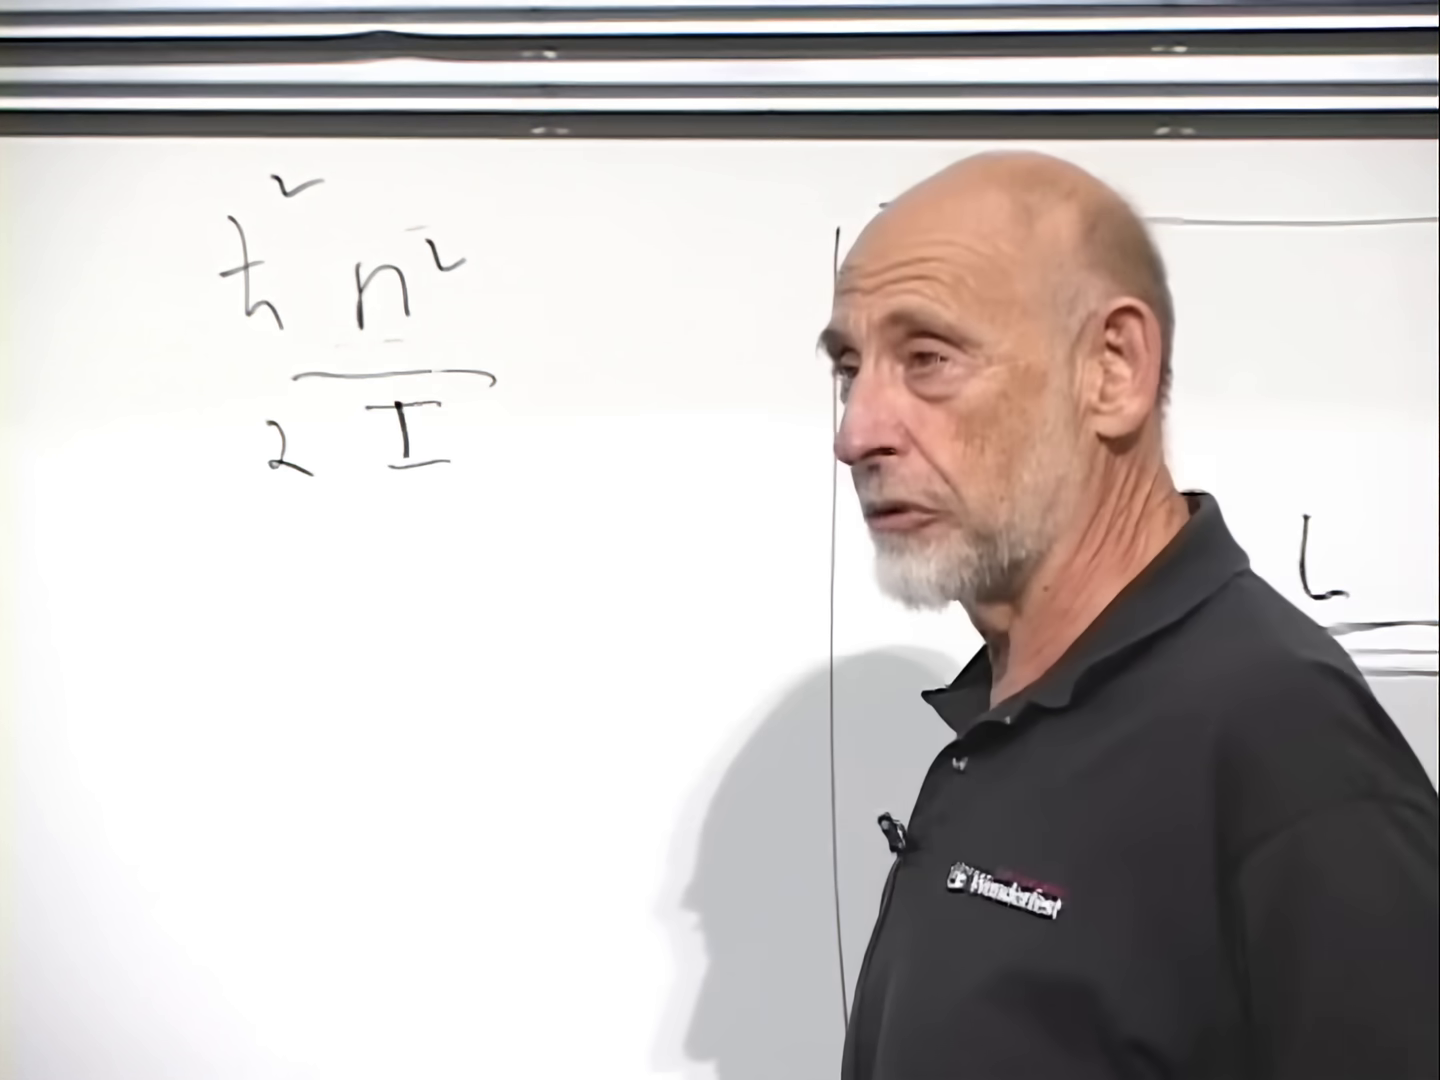
\includegraphics[width=0.76\textwidth]{lecture_01_figure_18.png}
  \caption{最初の回転励起に対する慣性モーメントの見積もり、\(\Delta E\sim\hbar^2/(2I)\)。}
  \lectureframe{01:44:00}
  \label{fig:l01-rotational-board}
\end{figure}

質量が一定なら、半径が小さいほど慣性モーメントははるかに小さくなり、励起エネルギーははるかに大きくなる。ハドロンはその内部力学の尺度では大きいため、回転励起に必要なエネルギーはおよそ一ギガ電子ボルトで、粒子衝突で到達できる。電子が何らかの空間的な内部構造をもつとしても、実験による制限から、その尺度ははるかに小さくなり、回転励起は利用可能なエネルギーを大幅に超えることになる。バスケットボールは逆の極端にある。慣性モーメントが非常に大きいため、角運動量一量子に必要なエネルギーは知覚できないほど小さい。原子の回転または軌道におけるエネルギーの段階はこの両極端の間にあり、通常は電子ボルトの尺度にある。

\begin{classroomqa}
\audiencequestion{一見素粒子に見える電子も、空間構造と回転励起をもちうるだろうか。\lecturetimestamp{01:42:04}}
\lecturerresponse{それは非常に高いエネルギーにおいてのみ、それらを隠しうる。角運動量1単位のコストは\(1/I\)としてスケールし、\(I\sim MR^2\)である。したがって、極端に小さい半径は、最初の励起を質量二乗プロット上ではるか遠くへ押しやる。観測された電子励起が存在しないことは、電子が点状であるか、あるいは複合性のスケールが現在の実験で分解できるよりもはるかに小さいかのいずれかを意味する。}
\end{classroomqa}

冒頭のレッジェプロットは、今や力学的に読むことができる。ハドロンは拡がっているため、アクセス可能な回転状態と振動状態を明らかにする。その質量二乗スペクトルにおける等間隔のステップは、振動子ハミルトニアンが\(M^2\)と同一視されるときに期待される特徴である。エネルギーが長さに対して近似的に線形であることは、一定の張力をもつフラックスチューブの特徴である。分光学、散乱の双対性、世界面の幾何学、光円錐力学は、同じ組織的アイデアの4つの記述である。すなわち、自然な内部変数が質量二乗である拡がった相対論的対象である。
